\chapter{Fibred categories, stacks, and moduli problems}
    \begin{abstract}
        
    \end{abstract}
    
    \minitoc
    
    \section{Fibred categories}
    \subsection{Generalities on \texorpdfstring{$2$}{}-categories}
        \subsubsection{\textit{Pr\'elude}: Internal categories}
            \begin{definition}[Spans] \label{def: spans} \index{Spans}
                \noindent
                \begin{enumerate}
                    \item \textbf{(Spans):} A \textbf{span} (also known as a \textbf{correspondence}) from an object $x$ to another object $y$ via an object $s$ inside a given category $\C$ is a diagram therein that is of the following form:
                        $$
                            \begin{tikzcd}
                            	s & y \\
                            	x
                            	\arrow["f"', from=1-1, to=2-1]
                            	\arrow["g", from=1-1, to=1-2]
                            \end{tikzcd}
                        $$
                    wherein the tip $s$ is some \textit{choice} of object of $\C$. As any span with either or both arrow therein being an identity is just a normal morphism, the notion of spans can be thought of as a generalisation of morphisms.  
                    \item \textbf{(Categories of spans):} Within a category $\C$ with pullbacks, one can compose, say, a span from $x$ to $y$ via $s$ with another from $y$ to $z$ via $s'$ via taking the pullback of the \say{inner} arrows in the manner depicted by the following diagram:
                        $$
                            \begin{tikzcd}
                            	{s \x_{g, y, f'} s'} & {s'} & z \\
                            	s & y \\
                            	x
                            	\arrow["f"', from=2-1, to=3-1]
                            	\arrow["g"', from=2-1, to=2-2]
                            	\arrow["{f'}", from=1-2, to=2-2]
                            	\arrow["{g'}", from=1-2, to=1-3]
                            	\arrow[from=1-1, to=2-1]
                            	\arrow[from=1-1, to=1-2]
                            	\arrow["\lrcorner"{anchor=center, pos=0.125}, draw=none, from=1-1, to=2-2]
                            \end{tikzcd}
                        $$
                    to obtain a so-called \say{composite} span from $x$ to $z$ via $s \x_{g, y, f'} s'$ (which visually, can be thought of either as the upper \say{roof} or the big \say{roof} covering the two smaller ones - that being the previously specified spans from $x$ to $y$ via $s$ and the span from $y$ to $z$ via $s'$ - in the above diagram); alternatively, one might visualise this composition via the following commutative diagram of spans:
                        $$
                            \begin{tikzcd}
                            	x & y & z
                            	\arrow["{(f,g)}", "\shortmid"{marking}, from=1-1, to=1-2]
                            	\arrow["{(f' g')}", "\shortmid"{marking}, from=1-2, to=1-3]
                            \end{tikzcd}
                        $$
                    With the use of this style of composition, one obtains, for every category $\C$ with pullbacks in tandem with a choice of natural number $n \geq 1$, a (lax) \textbf{$n$-category of spans} $\Span^{\leq n}(\C)$ that is defined via:
                        \begin{enumerate}
                            \item objects being those of $\C$ itself,
                            \item $1$-morphisms being spans between objects, which shall henceforth be known as $1$-spans,
                            \item and for all $2 \leq k \leq n$, $k$-morphisms, which shall henceforth be called $k$-spans, being $k$-cells between $(k-1)$-morphisms; for instance, a $2$-span between two $1$-spans is a commutative diagram of the following form:
                                $$
                                    \begin{tikzcd}
                                        \bullet \arrow[rd] \arrow[rdd, bend right] \arrow[rrd, bend left] &                             &         \\
                                                                                                          & \bullet \arrow[d] \arrow[r] & \bullet \\
                                                                                                          & \bullet                     &        
                                    \end{tikzcd}
                                $$
                        \end{enumerate}
                \end{enumerate}
            \end{definition}
            \begin{convention}[Regarding notations] \label{conv: span_notations}
                Obviously, writing out spans explicitly takes up a lot of effort and frankly, these diagrams can get confusing rather quickly. However, a quick observation tells us that because composites of spans are given by pullbacks, they actually satisfy the universal property of products taken in the arrow category of some given span category. That is to say, given an ambient category $\C$ with all pullbacks and two composable spans:
                    $$
                        \begin{tikzcd}
                        	& \bullet & \bullet \\
                        	\bullet & \bullet \\
                        	\bullet
                        	\arrow["f"', from=2-1, to=3-1]
                        	\arrow["g", from=2-1, to=2-2]
                        	\arrow["{f'}", from=1-2, to=2-2]
                        	\arrow["{g'}", from=1-2, to=1-3]
                        \end{tikzcd}
                    $$
                therein, their composite:
                    $$
                        \begin{tikzcd}
                        	\bullet & \bullet & \bullet \\
                        	\bullet & \bullet \\
                        	\bullet
                        	\arrow["f"', from=2-1, to=3-1]
                        	\arrow["g"', from=2-1, to=2-2]
                        	\arrow["{f'}", from=1-2, to=2-2]
                        	\arrow["{g'}", from=1-2, to=1-3]
                        	\arrow[from=1-1, to=2-1]
                        	\arrow[from=1-1, to=1-2]
                        	\arrow["\lrcorner"{anchor=center, pos=0.125}, draw=none, from=1-1, to=2-2]
                        \end{tikzcd}
                    $$
                is nothing but the product:
                    $$
                        \begin{tikzcd}
                        	{(f, g) \x (f', g')} & {(f', g')} \\
                        	{(f, g)}
                        	\arrow[dashed, from=1-1, to=2-1]
                        	\arrow[dashed, from=1-1, to=1-2]
                        \end{tikzcd}
                    $$
                in $\Mor\left(\Span^{\leq 1}(\C)\right)$ (which will probably be commonly written as $\Span^{\leq 1}(\C)_1$ from now on, so as to make the notion of spans fit snuggly into the language of internal categories, and also to cut back on parentheses) Therefore, our proposition of an alternative notation is as follows: the composition of two spans $(f, g)$ and $(f', g')$ shall instead be denoted by $(f, g) \x (f', g')$.
            \end{convention}
            \begin{convention}[Associators]
                Fix a \textit{weak} $n$-category $\C$, with $n \geq 1$. Now, for all $1 \leq k \leq n$ and all triples of \textit{composable} $(k - 1)$-morphisms $f, g, h$ of $\C$, let us call the $k$-cell:
                    $$(fg)h \to f(gh)$$
                (which we note to be invertible thanks to the weakness assumption on $\C$) a \textbf{$k$-associator}. An associator is called \textbf{trivial} if and only if it is an identity. See \href{https://ncatlab.org/nlab/show/associator}{\underline{here}} for more details. 
            \end{convention}
            \begin{remark}[Associators in span categories]
                Since pullbacks are merely unique up to unique isomorphisms, $k$-associators in the $n$-category $\Span^{\leq n}(\C)$ of spans of a given category $\C$ with pullbacks are generally non-trivial, but they are invertible. This implies that $n$-categories of spans are \textit{weak} $n$-categories, as opposed to simply being lax $n$-categories, but generally they are not strict $n$-categories. 
            \end{remark}
            
            \begin{proposition}[Limits and colimits of spans]
                
            \end{proposition}
        
            \begin{definition}[Internal categories] \label{def: internal_categories}
                Let $\E$ be a category with \textit{enough pullbacks}. A category \textbf{internal} to $\E$ is then a pair $(C_0, C_1)$ of objects of $\E$ defined via the following data:
                    \begin{enumerate}
                        \item \textbf{(Objects and morphisms):} An object of \textbf{objects} $C_0 \in \E$ and an object of \textbf{arrows} $C_1 \in \E$, both are to be viewed as internal analogues of the collections of objects and arrows in the definition of categories.
                        \item \textbf{(Composition):} 
                            \begin{enumerate}
                                \item \textbf{(Sources and targets):} From the object of arrows $C_1$ to the object of objects $C_0$, there are two morphisms $s, t$ as follows, known as the \textbf{source} and \textbf{target} maps:
                                    $$
                                        \begin{tikzcd}
                                        	{C_1} & {C_0}
                                        	\arrow["s", shift left=2, from=1-1, to=1-2]
                                        	\arrow["t"', shift right=2, from=1-1, to=1-2]
                                        \end{tikzcd}
                                    $$
                                which, respectively, assign to each arrow $f \in C_1$ (which, along with similar instances, shall be viewed as a \href{https://ncatlab.org/nlab/show/generalized+element}{\underline{generalised elements}} for the sake of linguistic convenience) its domain and codomain objects in $C_0$.
                                \item \textbf{(Units):} From the object of objects $C_0$ to the object of arrows $C_1$, there is a distinguished morphism:
                                    $$e: C_0 \to C_1$$
                                called the \textbf{unit map} which assigns to each object $x \in C_0$ (again, viewed as a generalised element) the identity $\id_x: x \to x$ thereon, which we note to be an a generalised element of the object of arrows $C_1$ (hence the codomain of $e$ is $C_1$).
                                \item \textbf{(Composition of arrows):} There is a monoidal composition operation (in the sense of monoidal categories):
                                    $$\mu: C_1 \x_{s, C_0, t} C_1 \to C_1$$
                                satisfying the following conditions specified by commutative diagrams in $\E$:
                                    \begin{enumerate}
                                        \item \textbf{(Identities do not alter domains and codomains):}
                                            $$
                                                \begin{tikzcd}
                                                	{C_0} & {C_1} && {C_0} & {C_1} \\
                                                	& {C_0} &&& {C_0}
                                                	\arrow["e", from=1-1, to=1-2]
                                                	\arrow["{\id_{C_0}}"', from=1-1, to=2-2]
                                                	\arrow["s", from=1-2, to=2-2]
                                                	\arrow["{\id_{C_0}}"', from=1-4, to=2-5]
                                                	\arrow["t", from=1-5, to=2-5]
                                                	\arrow["e", from=1-4, to=1-5]
                                                \end{tikzcd}
                                            $$
                                        \item \textbf{(Sources and targets of compositions):} The source of a composition $g \mu f \in C_1$ should be that of $f$ (the former), wheareas its target should be that of $g$ (the latter): 
                                            $$
                                                \begin{tikzcd}
                                                	& {C_1 \x_{s, C_0, t} C_1} & {C_1} && {C_1 \x_{s, C_0, t} C_1} & {C_1} \\
                                                	{} & {C_1} & {C_0} && {C_1} & {C_0}
                                                	\arrow["s", from=1-3, to=2-3]
                                                	\arrow["s", from=2-2, to=2-3]
                                                	\arrow["{\pr_2}"', from=1-2, to=2-2]
                                                	\arrow["{\pr_1}", from=1-2, to=1-3]
                                                	\arrow["t", from=1-6, to=2-6]
                                                	\arrow["t", from=2-5, to=2-6]
                                                	\arrow["{\pr_1}"', from=1-5, to=2-5]
                                                	\arrow["{\pr_1}", from=1-5, to=1-6]
                                                \end{tikzcd}
                                            $$
                                        \item \textbf{(Associativity):} 
                                            $$
                                                \begin{tikzcd}
                                                	& {C_1 \x_{s, C_0, t} C_1 \x_{s, C_0, t} C_1} & {C_1 \x_{s, C_0, t} C_1} \\
                                                	{} & {C_1 \x_{s, C_0, t} C_1} & {C_1}
                                                	\arrow["\mu", from=1-3, to=2-3]
                                                	\arrow["\mu", from=2-2, to=2-3]
                                                	\arrow["{\id_{C_1} \x_{s, C_0, t} \mu}"', from=1-2, to=2-2]
                                                	\arrow["{\mu \x_{s, C_0, t} \id_{C_1}}", from=1-2, to=1-3]
                                                \end{tikzcd}
                                            $$
                                        \item \textbf{(Left and right-unitarity):} 
                                    \end{enumerate}
                                        $$
                                            \begin{tikzcd}
                                            	{C_0 \x_{C_0} C_1} & {C_1 \x_{s, C_0, t} C_1} & {C_1 \x_{C_0} C_0} \\
                                            	& {C_1}
                                            	\arrow["\mu", from=1-2, to=2-2]
                                            	\arrow["{\pr_2}"', from=1-1, to=2-2]
                                            	\arrow["{\pr_1}", from=1-3, to=2-2]
                                            	\arrow["{\e \x_{C_0} \id_{C_1}}", from=1-1, to=1-2]
                                            	\arrow["{\id_{C_1} \x_{C_0} e}"', from=1-3, to=1-2]
                                            \end{tikzcd}
                                        $$
                                with the latter three specifying the monoidality of the composition operation $\mu$.
                            \end{enumerate}
                    \end{enumerate}
            \end{definition}
            
            \begin{remark}[Internal categories vs. subcategories]
                    
            \end{remark}
            
            \begin{remark}[Another formulation: Internal categories as monads on spans] \label{remark: internal_categories_alt_def}
                Definition \ref{def: internal_categories} gives us a perfectly fine idea of what one might mean by \say{internal categories}. However, it is manifestly rather clunky. Therefore, the author has taken the liberty to provide one alternative formulation of the notion of internal categories.
                
                We refer the reader to definition \ref{def: spans} and the discussion that follows for necessary information on the paradigm of spans; in particular, let us recall that spans are only well-defined inside categories with pullbacks (which is a slightly stronger condition than the assumption in definition \ref{def: internal_categories} that the ambient category as merely \textit{enough} pullbacks). 
                    
                Now, let $\E$ be an ambient category with all pullbacks, and subsequently, let us define a category $C$ internal to $\E$ as being the same as a monad in the weak $2$-category $\Span^{\leq 2}(\E)$ of spans on $\E$. Why would this even resemble a reasonable definition of categories internal to a given category $\E$ ? For starters, recall that a monad is an endomorphism satisfying so-called \say{monoidal multiplication}. Therefore, an internal category $C$ inside a given ambient category $\E$ is first and foremost an endomorphism on a choice of object, and because the weak $2$-category in which we are trying to build monads is one of spans, our endomorphism should be a \say{roof} diagram whose two \say{lower} vertices are the same. By consulting definition \ref{def: internal_categories}, one sees that an obvious choice is the source-target span:
                    $$
                        \begin{tikzcd}
                        	{C_1} & {C_0} \\
                        	{C_0}
                        	\arrow["s"', from=1-1, to=2-1]
                        	\arrow["t", from=1-1, to=1-2]
                        \end{tikzcd}
                    $$
                (recall that objects in span categories are those of the underlying category and morphisms are span themselves; cf. definition \ref{def: spans}); let us denote this span by the \textit{unordered} pair $(s, t)$. Now, is this endomorphism indeed a monad in $\Span^{\leq 2}(\E)$ ? First of all, one can certainly compose $(s, t)$ with itself thanks to the assumption that $\E$ has all pullbacks: said composition is nothing but the composite span $(s, t) \x (s, t)$ (see remark \ref{conv: span_notations} for an explanation of this notation); let us denote this composition by $\mu$, and note that it is precisely a $2$-cell from $(s, t) \x (s, t)$ to $(s, t)$, a fact that can be proven via consideration of the following universal diagram:
                    $$
                        \begin{tikzcd}
                        	{(s, t) \x (s, t)} & {(s, t)} \\
                        	{(s, t)} & {(s, t)}
                        	\arrow[dashed, from=1-1, to=2-1]
                        	\arrow[dashed, from=1-1, to=1-2]
                        	\arrow[Rightarrow, no head, from=1-2, to=2-2]
                        	\arrow[Rightarrow, no head, from=2-1, to=2-2]
                        	\arrow["\mu", from=1-1, to=2-2]
                        \end{tikzcd}
                    $$
                and thanks to the universal property of products, this composition is trivially asociative. There is also a unit $e := (\id_{C_0}, \id_{C_0}) \x (s, t)$ which satisfies the following commutative diagram:
                    $$
                        \begin{tikzcd}
                        	{(\id_{C_0}, \id_{C_0}) \x (s, t)} & {(s, t) \x (s, t)} & {(s, t) \x (\id_{C_0}, \id_{C_0})} \\
                        	& {(s, t)}
                        	\arrow["\mu", from=1-2, to=2-2]
                        	\arrow["{\pr_2}"', from=1-1, to=2-2]
                        	\arrow["{\pr_1}", from=1-3, to=2-2]
                        	\arrow["{e \x \id_{(s, t)}}", from=1-1, to=1-2]
                        	\arrow["{\id_{(s, t)} \x e}"', from=1-3, to=1-2]
                        \end{tikzcd}
                    $$
                This proves that the composition $\mu$ is also unital, and hence all the monad axioms have been shown to hold. Incidentally, we have also managed to show via this discussion, that monads in the category of spans in a category with pullbacks are nothing but internal categories.
            \end{remark}
            
            \begin{definition}[Internal functors] \label{def: internal_functors}
                Let $\E$ be an ambient category with \textit{enough pullbacks} and let $C, D$ be two categories that are internal to $\E$.
                    \begin{enumerate}
                        \item \textbf{(Internal functors):} Internal functors between categories that are internal to a given ambient category (with enough pullbacks) are defined in the exact same way as the internal definition of functors between ordinary categories. See \href{https://ncatlab.org/nlab/show/functor#InternalDefinition}{\underline{here}} for a reminder.
                        \item \textbf{(Anafunctors):} (Ah yes, the Axiom of Choice. Making lives miserable as always) While the general definition of internal functors might not have lit any bulbs in the deparment of choice, one should definitely keep in mind that the notion of essential surjectivity definitely does depend on choice: if:
                            $$F: C \to D$$
                        is an essentially surjective internal functor, then one will be able to \textit{choose} objects $x \in C_0$ such that:
                            $$Fx \cong y$$
                        for every object $y \in D_0$. As the ramifications of the Axiom of Choice tend to be unfamiliar to those not actively involved in the logic community (including the author, who had to consult a few nLab articles too), let us quickly explain why anafunctors are needed in place of the above \textit{na\"ive} notion of internal functors; particularly, we would like to know what mappings between internal categories might look like when our ambient category does not host the Axiom of Choice, such as when its size is an inaccessible cardinal ($\Top$ is one particular case). To that end, \todo[inline]{Write about why the Axiom of Choice breaks essentially surjective internal functors}
                        
                        Now, let us define an \textbf{anafunctor} $F$ between two internal categories $C$ and $D$ of a given category $\E$ - should such a mapping exist - to be a span (i.e. a $1$-morphism in $\Span^{\leq 2}(\E)$; cf. definition \ref{def: spans}) of internal categories:
                            $$
                                \begin{tikzcd}
                                	{F} & {D} \\
                                	{C}
                                	\arrow[from=1-1, to=2-1]
                                	\arrow[from=1-1, to=1-2]
                                \end{tikzcd}
                            $$
                        which shall be interpreted as the following composition of spans in $\E$:
                            $$
                                \begin{tikzcd}
                                	\bullet & \bullet & {D_1} & {D_0} \\
                                	\bullet & {F_0} & {D_0} \\
                                	{C_1} & {C_0} \\
                                	{C_0}
                                	\arrow[from=3-1, to=4-1]
                                	\arrow[from=3-1, to=3-2]
                                	\arrow[from=2-2, to=3-2]
                                	\arrow[from=2-2, to=2-3]
                                	\arrow[from=1-3, to=2-3]
                                	\arrow[from=1-3, to=1-4]
                                	\arrow[from=2-1, to=3-1]
                                	\arrow[from=2-1, to=2-2]
                                	\arrow[from=1-1, to=2-1]
                                	\arrow[from=1-1, to=1-2]
                                	\arrow[from=1-2, to=2-2]
                                	\arrow[from=1-2, to=1-3]
                                	\arrow["\lrcorner"{anchor=center, pos=0.125}, draw=none, from=1-2, to=2-3]
                                	\arrow["\lrcorner"{anchor=center, pos=0.125}, draw=none, from=1-1, to=2-2]
                                	\arrow["\lrcorner"{anchor=center, pos=0.125}, draw=none, from=2-1, to=3-2]
                                \end{tikzcd}
                            $$
                        (see remark \ref{remark: internal_categories_alt_def} for a description of internal categories as spans - or to be more precise, monads in span categories). Note that in the event that $\E$ also has products (or equivalently, terminal objects), anafunctors between any given pair of internal categories $C$ and $D$ always exist: one can simply take $F_0$ to be $C_0 \x D_0$. Also, let us draw attention to the fact that this definition is logically independent of the notion of internal functors, and therefore we have not committed circular reasoning.
                    \end{enumerate}
            \end{definition}
            \begin{remark}[Categories of internal categories] \label{remark: categories_of_internal_categories}
                Via the above notion of anafunctors and the idea presented in remark \ref{remark: internal_categories_alt_def} that internal categories and monads in span categories are the same thing, one can rather easily show that categories internal to a given ambient category $\E$ (with pullbacks) form a weak $2$-category, which is precisely equivalent to the category of monads in $\Span^{\leq 2}(\E)$. In notations, one writes:
                    $$1\-\Cat(\E) \cong \Monad\left(\Span^{\leq 2}(\E)\right)$$
            \end{remark}
            \begin{remark}[Categories as monoids] \label{remark: categories_as_monoids}
                Remark \ref{remark: internal_categories_alt_def}, definition \ref{def: internal_functors}, remark \ref{remark: categories_of_internal_categories}, and remark \ref{conv: span_notations} in tandem tell us that internal to every ambient category $\E$ with pullbacks, there is a symmetric monoidal category $1\-\Cat(\E)$ of categories internal to $\E$ whose monoidal multiplication is given by $2$-spans from squares:
                    $$
                        \begin{tikzcd}
                        	{C_1 \x_{s, C_0, t} C_1} \\
                        	& {C_1} & {C_0} \\
                        	& {C_0}
                        	\arrow["s", from=2-2, to=3-2]
                        	\arrow["t"', from=2-2, to=2-3]
                        	\arrow[from=1-1, to=3-2]
                        	\arrow[from=1-1, to=2-3]
                        	\arrow["\mu"{description}, from=1-1, to=2-2]
                        \end{tikzcd}
                    $$
                and whose monoidal unit is given pointwise on each internal category:
                    $$
                        \begin{tikzcd}
                        	{C_1} & {C_0} \\
                        	{C_0}
                        	\arrow["s"', from=1-1, to=2-1]
                        	\arrow["t", from=1-1, to=1-2]
                        \end{tikzcd}
                    $$
                by a $2$-span from $(\id_{C_0}, \id_{C_0}) \to (s,t)$:
                    $$
                        \begin{tikzcd}
                        	{C_0} \\
                        	& {C_1} & {C_0} \\
                        	& {C_0}
                        	\arrow["s", from=2-2, to=3-2]
                        	\arrow["t"', from=2-2, to=2-3]
                        	\arrow["e"{description}, from=1-1, to=2-2]
                        	\arrow["{\id_{C_0}}"', from=1-1, to=3-2]
                        	\arrow["{\id_{C_0}}", from=1-1, to=2-3]
                        \end{tikzcd}
                    $$
                Both of which (together) are subjected to the usual monoidal axioms (cf. definition \ref{def: internal_categories}). In other words, internal categories inside a given ambient category $\E$ are nothing but monoids in $1\-\Cat(\E)$. This is a rather neat observation, as it allows us to view morphisms between internal categories not too differently from monoid homomorphism. 
            \end{remark}
            
            \begin{definition}[Internal groupoids] \label{def: internal_groupoids}
                Let $\E$ be a category with pullbacks and let:
                    $$
                        \begin{tikzcd}
                        	{\scrG_1} & {\scrG_0} \\
                        	{\scrG_0}
                        	\arrow["s"', from=1-1, to=2-1]
                        	\arrow["t", from=1-1, to=1-2]
                        \end{tikzcd}
                    $$
                be the data of a category internal to $\E$. Such an internal category is an \textbf{internal groupoid} if in addition, there exists an arrow:
                    $$i: \scrG_1 \to \scrG_1$$
                called the \textbf{inverse map}, that renders the following diagram in $\E$ commutative:
                    $$
                        \begin{tikzcd}
                        	{\scrG_1} \\
                        	& {\scrG_1} & {\scrG_0} \\
                        	& {\scrG_0}
                        	\arrow["i"{description}, from=1-1, to=2-2]
                        	\arrow["t"', from=1-1, to=3-2]
                        	\arrow["s", from=2-2, to=3-2]
                        	\arrow["t"', from=2-2, to=2-3]
                        	\arrow["s", from=1-1, to=2-3]
                        \end{tikzcd}
                    $$
                (i.e. the inverse map switches the source and target of a given internal morphism), and such that the following diagrams of spans - telling us that multiplication with inverses returns the identity regardless of whether the process is carried out from the left and from the right - commute:
                    $$
                        \begin{tikzcd}
                        	{\scrG_1} & {\scrG_1 \x_{s, \scrG_0, t} \scrG_1} & {\scrG_1 \x_{s, \scrG_0, t} \scrG_1} \\
                        	{\scrG_0} && {\scrG_1}
                        	\arrow["{\mu_{\scrG}}", from=1-3, to=2-3]
                        	\arrow["{i \x_{s, \scrG_0, t} \id_{\scrG_1}}", from=1-2, to=1-3]
                        	\arrow["{\Delta_{\scrG_1/\scrG_0}}", from=1-1, to=1-2]
                        	\arrow["t"', from=1-1, to=2-1]
                        	\arrow["e", from=2-1, to=2-3]
                        \end{tikzcd}
                    $$
                    $$
                        \begin{tikzcd}
                        	{\scrG_1} & {\scrG_1 \x_{s, \scrG_0, t} \scrG_1} & {\scrG_1 \x_{s, \scrG_0, t} \scrG_1} \\
                        	{\scrG_0} && {\scrG_1}
                        	\arrow["{\mu_{\scrG}}", from=1-3, to=2-3]
                        	\arrow["{\id_{\scrG_1} \x_{s, \scrG_0, t} i}", from=1-2, to=1-3]
                        	\arrow["{\Delta_{\scrG_1/\scrG_0}}", from=1-1, to=1-2]
                        	\arrow["s"', from=1-1, to=2-1]
                        	\arrow["e", from=2-1, to=2-3]
                        \end{tikzcd}
                    $$
                In other words, groupoids internal to a category with pullbacks $\E$ are group objects in the category $1\-\Cat(\E)$ of categories internal to $\E$ (which we note to have all finite products; cf. remark \ref{conv: span_notations}).
            \end{definition}
            \begin{remark}[On the inverse maps of internal groupoids]
                Definition \ref{def: internal_groupoids}, while standard, suffers from a few issues. For one, it is not very clear how internal groupoids should be thought of as groups in categories of internal categories. Also, the inverse map defining the structure of each internal groupoid, at least according to definition \ref{def: internal_groupoids}, is rather non-functorial. Luckily, these two problems can be easily resolved. 
                
                Firstly, let us note that the inverse map $i_{\scrG}: \scrG_1 \to \scrG_1$ associated to an internal groupoid:
                    $$
                        \begin{tikzcd}
                        	{\scrG_1} & {\scrG_0} \\
                        	{\scrG_0}
                        	\arrow["s"', from=1-1, to=2-1]
                        	\arrow["t", from=1-1, to=1-2]
                        \end{tikzcd}
                    $$
                is not just a morphism in the ambient category satisfying certain conditions, but actually a $2$-span: it is a $2$-span from the $1$-span $(s,t): \scrG_1 \toto \scrG_0$ to the $1$-span $(t,s): \scrG_1 \toto \scrG_0$. Thus, one can meaningfully think of the inverse map on $\scrG$ as an anafunctor from $\scrG$ to itself. Second of all, recall that in remark \ref{remark: categories_as_monoids}, we have seen how internal categories are actually monoid objects, which in particular, means that composition of arrows therein behaves in a manner similar to multiplication. So actually, all that we need to do is to somehow configure inverse maps so that they would act like multiplicative inverses, which would in turn help us formally recognise internal groupoids as group objects; we shall leave the drawing of the relevant commutative diagrams to the reader, as they can be rather easily inferred from the ones in definition \ref{def: internal_groupoids}. 
            \end{remark}
        
            \begin{definition}[Equivalence relations] \label{def: equivalence_relations}
                Let $\E$ be a \textit{finitely complete} category ($\Sets$ or general topoi, or $1\-\Cat$, for instance)
                    \begin{enumerate}
                        \item \textbf{(Binary relations):} A \textbf{binary relation} $R$ from an object $X$ to another object $Y$ of $\E$ is a $1$-span:
                            $$
                                \begin{tikzcd}
                                	R & Y \\
                                	X
                                	\arrow[from=1-1, to=2-1]
                                	\arrow[from=1-1, to=1-2]
                                \end{tikzcd}
                            $$
                        such that $R$ is a subobject of $X \x Y$. 
                        \item \textbf{(Equivalence relations):} An \textbf{equivalence relation} (also known as a congruence) $R$ on an object $X$ of $\E$ is a binary relation from $X$ to itself which also happens to be an internal groupoid. 
                        \item \textbf{(Quotients):} The coequaliser of an (internal) equivalence relation is known as a \textbf{quotient object}. That is, the quotient $Q$ of an object $X$ by an equivalence relation $R$ is the following coequaliser in $\E$:
                            $$
                                \begin{tikzcd}
                                	R & X & Q
                                	\arrow["s", shift left=2, from=1-1, to=1-2]
                                	\arrow["t"', shift right=2, from=1-1, to=1-2]
                                	\arrow[dashed, from=1-2, to=1-3]
                                \end{tikzcd}
                            $$
                        Of course, quotients are only guaranteed to exist if and only if $\E$ has enough coequalisers. 
                    \end{enumerate}
            \end{definition}
        
        \subsubsection{\texorpdfstring{$2$}{}-categorical constructions}
            \begin{definition}[$2$-categories and $2$-functors] \label{def: 2_categories_and_2_functors}
                
            \end{definition}
            \begin{definition}[$(2, k)$-categories] \label{def: (2, k)_categories} 
                A $(2, k)$-category (for $0 \leq k \leq 2$) is a $2$-category wherein all $(k + 1)$-morphisms are invertible.
            \end{definition}
            \begin{definition}[$2$-natural transformations] \label{def: 2_natural_transformations}
                
            \end{definition}
            \begin{definition}[Natural modifications] \label{def: natural_modifications}
                
            \end{definition}
            \begin{remark}[$2$-categories of $2$-functors] \label{remark: 2_categories_of_2_functors}
                
            \end{remark}
            
            \begin{definition}[$2$-commutative diagrams] \label{def: 2_commutative_diagrams}
                Let $\scrK$ be a $2$-category. A $2$-commutative diagram therein is thus a square as follows, wherein there exists a $2$-isomorphism $\eta: p'f \Rightarrow pg$:
                    $$
                        \begin{tikzcd}
                        	{y'} & y \\
                        	{x'} & x
                        	\arrow["{p'}"', from=1-1, to=2-1]
                        	\arrow["f", from=2-1, to=2-2]
                        	\arrow["g", from=1-1, to=1-2]
                        	\arrow["p", from=1-2, to=2-2]
                        	\arrow["\exists \eta", shorten <=8pt, shorten >=8pt, Rightarrow, from=2-1, to=1-2]
                        \end{tikzcd}
                    $$
            \end{definition}
            
            \begin{definition}[Strict and weak $2$-categories and $2$-functors] \label{def: strict_and_weak_2_categoriesand_2_functors}
                \noindent
                \begin{enumerate}
                    \item \textbf{(Strict and weak $2$-categories):} Let $\scrK$ be a $2$-category. One says that it is \textbf{strict} if compositions of (pairs of) $1$-morphisms are unique up to (necessarily unique) $2$-equalities, and \textbf{weak} if compositions of (pairs of) $1$-morphisms are unique only up to $2$-isomorphisms.
                    \item \textbf{(Strict and weak $2$-functors):}
                \end{enumerate}
            \end{definition}
            \begin{example}
                
            \end{example}
            
            Strictly speaking, the following notion ought to be known as that of $(2, 1)$-pullbacks, but since we shall not be encountering so-called \say{\textit{lax} $2$-pullbacks} (or any lax $2$-(co)limits for that matter), we shall be lazy and simply write \say{$2$-pullbacks} to mean \say{$(2, 1)$-pullbacks}.
            \begin{definition}[$2$-pullbacks] \label{def: 2_pullbacks}
                
            \end{definition}
            \begin{example}[$2$-pullbacks in $1\-\Cat_2$] \label{example: 2_pullbacks_in_the_2_category_of_categories}
                The $2$-category $1\-\Cat_2$ whose objects are $1$-categories, whose $1$-morphisms are functors, and whose $2$-morphisms are natural transformations, has all $2$-pullbacks.
            \end{example}
    
    \subsection{(Co)fibred categories}
        \subsubsection{Slice \texorpdfstring{$2$}{}-categories and prefibrations}
            \begin{definition}[Slice $2$-categories] \label{def: slice_2_categories}
                Let $\scrK$ be a $2$-category and let $x \in \Ob(\scrK)$ be an object therein. Then, we define the \textbf{slice} $2$-category $\scrK_{/x}$ to be the $2$-category wherein:
                    \begin{itemize}
                        \item the objects are $1$-morphisms $(f: y \to x) \in 1\-\Mor(\scrK)$,
                        \item the $1$-morphisms $\varphi: (y', f') \to (y, f)$ are $1$-commutative triangles of $1$-morphisms $(f': y' \to x), (f: y \to x) \in 1\-\Mor(\scrK)$ in $\scrK$ of the following form:
                            $$
                                \begin{tikzcd}
                                	{y'} && y \\
                                	& x
                                	\arrow["\varphi", from=1-1, to=1-3]
                                	\arrow["{f'}"', from=1-1, to=2-2]
                                	\arrow["f", from=1-3, to=2-2]
                                \end{tikzcd}
                            $$
                        \item and the $2$-morphisms between $1$-morphisms $\varphi, \psi: (y', f') \to (y, f)$ are $2$-morphisms $(\eta: \psi \Rightarrow \varphi) \in 2\-\Mor(\scrK)$ such that the following diagram is $2$-commutative:
                            $$
                                \begin{tikzcd}
                                	{y'} && y \\
                                	& x
                                	\arrow["{f'}"', from=1-1, to=2-2]
                                	\arrow["f", from=1-3, to=2-2]
                                	\arrow[""{name=0, anchor=center, inner sep=0}, "\varphi"', bend right, from=1-1, to=1-3]
                                	\arrow[""{name=1, anchor=center, inner sep=0}, "\psi", bend left, from=1-1, to=1-3]
                                	\arrow["\eta"', shorten <=3pt, shorten >=3pt, Rightarrow, from=1, to=0]
                                \end{tikzcd}
                            $$
                    \end{itemize}
            \end{definition}
            \begin{example}[Over-categories] \label{example: over_categories}
                Let $\C$ be a category and let $1\-\Cat_2$ be the $2$-category with $1$-categories, functors, and natural transformations as objects, $1$-morphisms, and $2$-morphisms respectively. Then, there is a natural slice $2$-category $(1\-\Cat_2)_{/\C}$ wherein the objects are functors $p: \scrS \to \C$, $1$-morphisms are the evident $1$-commutative triangles of functors, and $2$-morphisms between $1$-morphisms $F, G: (\scrS', p') \to (\scrS, p)$ are natural transformations $\eta \in \Nat(F, G)$ such that $p(\eta_y) \cong \id_{p'(y)}$ for all $y \in \Ob(\scrS')$, i.e. such that the following square is $2$-commutative:
                    $$
                        \begin{tikzcd}
                        	{p'(y)} & {p(F(y))} \\
                        	{p'(y)} & {p(G(y))}
                        	\arrow["{p(\eta_y)}", from=1-2, to=2-2]
                        	\arrow[from=1-1, to=1-2]
                        	\arrow["{\id_{p'(y)}}"', from=1-1, to=2-1]
                        	\arrow[from=2-1, to=2-2]
                        	\arrow[shorten <=8pt, shorten >=8pt, Rightarrow, from=2-1, to=1-2]
                        \end{tikzcd}
                    $$
            \end{example}
            \begin{proposition}[$2$-pullbacks in slice $2$-categories] \label{prop: 2_pullbacks_in_slice_2_categories}
                Let $\scrK$ be a $2$-category with $2$-pullbacks. Then for any $x \in \Ob(\scrK)$, the slice $2$-category $\scrK_{/x}$ shall also possess all $2$-pullbacks.
            \end{proposition}
                \begin{proof}
                            
                \end{proof}
            \begin{corollary}[$2$-pullbacks of over-categories] \label{coro: 2_pullbacks_of_over_categories}
                If $\C$ is any $1$-category then the $2$-category $(1\-\Cat_2)_{/\C}$ will have all $2$-pullbacks.
            \end{corollary}
            
            \begin{definition}[Prefibrations] \label{def: prefibrations}
                Consider a $1$-functor $p: \scrS \to \C$ between $1$-categories $\scrS$ and $\C$ is a \textbf{prefibration} if and only if it is surjective on the level of both objects and ($1$-)morphisms. 
            \end{definition}
            \begin{remark}[Op-prefibrations] \label{remark: op_prefibrations}
                It is easy to see that every prefibration $p: \scrS \to \C$ defines a so-called \textbf{op-prefibration} $p^{\op}: \scrS^{\op} \to \C^{\op}$, which is nothing but the functor $p^{\op}$ viewed as a prefibration of $\scrS^{\op}$ over $\C^{\op}$.
            \end{remark}
            \begin{remark}[Fibres of prefibrations] \label{remark: fibres_of_prefibrations}
                Consider a prefibration $p: \scrS \to \C$, viewed as a $1$-morphism of $1\-\Cat_2$, and recall that $1\-\Cat_2$ admits $1$-terminal objects, namely categories that are equivalent to the singleton category $\pt$, as well as $2$-pullbacks. By viewing objects $U \in \Ob(\C)$ as functors $U: \pt \to \C$, one can define \textbf{fibres} of the prefibration $p: \scrS \to \C$ as $2$-pullbacks of the following kind:
                    $$
                        \begin{tikzcd}
                        	{\scrS_U} & \scrS \\
                        	\pt & \C
                        	\arrow["U", from=2-1, to=2-2]
                        	\arrow["p", from=1-2, to=2-2]
                        	\arrow["{p_U}"', from=1-1, to=2-1]
                        	\arrow[from=1-1, to=1-2]
                        	\arrow["2"{description}, "\lrcorner"{anchor=center, pos=0.125}, draw=none, from=1-1, to=2-2]
                        \end{tikzcd}
                    $$
                It is then easy to see that $\scrS_U$ is the category wherein the objects are objects $x \in \scrS$ such that $p(x) = U$ and the morphisms are morphisms $(\varphi: y \to x) \in \Mor(\scrS)$ such that $p(\varphi) = \id_U$, and as such one ought to view $p_U: \scrS_U \to \pt$ as the unique functor from $\scrS_U$ to the singleton category whose only object is $U$ and whose only morphism is $\id_U$. Therefore, one can instead define prefibrations as functors $p: \scrS \to \C$ with non-empty fibres in the sense above and identify them by the families of $2$-pullbacks $\{\scrS \x^2_{p, \C, U} \pt\}_{U \in \Ob(\C)}$.
            \end{remark}
            \begin{remark}[The $2$-category of prefibrations]
                By definition, prefibrations $p: \scrS \to \C$ are objects of the $2$-category $(1\-\Cat_2)_{/\C}$, and so we might be tempted to declare that there is a $2$-full subcategory $\Pre\Fib(\C) \overset{2}{\subset} (1\-\Cat_2)_{/\C}$ spanned by prefibrations over $\C$, and indeed there is. To check that this is the case, one can verify that given any $1$-morphism $(F: (\scrS', p') \to (\scrS, p)) \in 1\-\Mor((1\-\Cat_2)_{/\C})$ and any object $U \in \C$, there exists a functor $F_U: \scrS'_U \to \scrS_U$ making the following diagram $2$-commutative in $1\-\Cat_2$:
                    $$
                        \begin{tikzcd}
                        	{\scrS'_U} &&&& {\scrS_U} \\
                        	{\scrS'} &&&& \scrS \\
                        	&& \pt \\
                        	&& \C
                        	\arrow["{p'}"', from=2-1, to=4-3]
                        	\arrow["U", from=3-3, to=4-3]
                        	\arrow["{p'_U}"', from=1-1, to=3-3]
                        	\arrow["\lrcorner"{anchor=center, pos=0.125}, draw=none, from=1-1, to=4-3, "2"{description}]
                        	\arrow[from=1-1, to=2-1]
                        	\arrow["{p_U}", from=1-5, to=3-3]
                        	\arrow[from=1-5, to=2-5]
                        	\arrow["p", from=2-5, to=4-3]
                        	\arrow["F", from=2-1, to=2-5]
                        	\arrow["{F_U}", from=1-1, to=1-5, dashed]
                        	\arrow["\lrcorner"{anchor=center, pos=0.125, rotate=-90}, draw=none, from=1-5, to=4-3, "2"{description}]
                        \end{tikzcd}
                    $$
                and similarly for $2$-morphisms in $\Pre\Fib(\C)$. We leave this as an exercise for the reader, for which they may make use of proposition \ref{prop: 2_pullbacks_in_slice_2_categories}. Via the Pasting Lemma for $2$-pullbacks, we also see that:
                    $$\scrS'_U \cong \scrS' \x^2_{F, \scrS} \scrS_U$$
                from which it is easy to deduce that $\Pre\Fib(\C)$ has all $2$-pullbacks.
            \end{remark}
        
        \subsubsection{(Co)cartesian arrows and (co)fibrations of categories; prestacks}
            \begin{definition}[(Co)cartesian arrows] \label{def: (co)cartesian_arrows}
                Consider a prefibration $p: \scrS \to \C$. Then, an arrow $(\varphi: y \to x) \in \Mor(\scrS)$ is said to be \textbf{$p$-cartesian} if and only if for all objects $z \in \Ob(\scrS)$, one has a ($1$-)pullback square of the following form:
                    $$
                        \begin{tikzcd}
                        	{\scrS(z, y)} & {\C(p(z), p(y))} \\
                        	{\scrS(z, x)} & {\C(p(z), p(x))}
                        	\arrow["{\scrS(z, \varphi)}"', from=1-1, to=2-1]
                        	\arrow[from=2-1, to=2-2]
                        	\arrow["{\C(p(z), p(\varphi))}", from=1-2, to=2-2]
                        	\arrow[from=1-1, to=1-2]
                        	\arrow["\lrcorner"{anchor=center, pos=0.125}, draw=none, from=1-1, to=2-2]
                        \end{tikzcd}
                    $$
                Dually, the given arrow $\varphi: y \to x$ is \textbf{$p$-cocartesian} if and only if it is $p^{\op}$-cartesian.
            \end{definition}
            \begin{remark}[Weakly (co)cartesian arrows ?] \label{remark: weak_(co)cartesian_arrows}
                
            \end{remark}
            \begin{proposition}[Properties of (co)cartesian arrows in a prefibration] \label{prop: properties_of_(co)cartesian_arrows_in_a_prefibration}
                Let $p: \scrS \to \C$ be a prefibration. Then:
                    \begin{enumerate}
                        \item compositions of $p$-(co)cartesian arrows are also $p$-(co)cartesian,
                        \item isomorphisms in $\scrS$ are $p$-(co)cartesian, 
                        \item if a $p$-(co)cartesian arrow $(\varphi: y \to x) \in \Mor(\scrS)$ is such that $p(\varphi)$ is an isomorphism in $\C$, then $\varphi$ itself will be an isomorphism, and
                        \item if we have a diagram in $\scrS$ as follows, wherein $\varphi: y \to x$ is $p$-(co)cartesian:
                            $$
                                \begin{tikzcd}
                                	& y \\
                                	{x'} & x
                                	\arrow["\varphi", from=1-2, to=2-2]
                                	\arrow["f", from=2-1, to=2-2]
                                \end{tikzcd}
                            $$
                        such that the pullback $p(y) \x_{p(\varphi), p(x), p(f)} p(x')$ exists in $\C$, then the pullback $y \x_{\varphi, x, f} x'$ exists in $\scrS$, and moreover, the canonical projection $\pr_1: y \x_{\varphi, x, f} x' \to x'$ is also $p$-(co)cartesian.
                    \end{enumerate}
            \end{proposition}
                \begin{proof}
                    \noindent
                    \begin{enumerate}
                        \item 
                        \item 
                        \item 
                        \item 
                    \end{enumerate}
                \end{proof}
            \begin{proposition}[(Co)cartesian arrows under $1$-morphisms of prefibrations] \label{prop: (co)cartesian_arrows_under_1_morphisms_of_prefibrations}
                Let $\C$ be a base category and consider a $1$-morphism in $\Pre\Fib(\C)$ as follows:
                    $$
                        \begin{tikzcd}
                        	{\scrS'} && \scrS \\
                        	& \C
                        	\arrow["{p'}"', from=1-1, to=2-2]
                        	\arrow["p", from=1-3, to=2-2]
                        	\arrow["F", from=1-1, to=1-3]
                        \end{tikzcd}
                    $$
                If $(\psi: z \to t) \in \Mor(\scrS')$ is a $p'$-(co)cartesian arrow such that $F(\psi)$ is $p$-(co)cartesian, then $\psi$ will be $(F \circ p)$-(co)cartesian. 
            \end{proposition}
                \begin{proof}
                    Immediate from definition \ref{def: (co)cartesian_arrows}.
                \end{proof}
            
            \begin{definition}[(Op)fibrations] \label{def: (op)fibrations}
                A \textbf{fibration}\footnote{Also called a \textbf{fibred category} or \textbf{cartesian fibration}.} is a prefibration $p: \scrS \to \C$ such that for all arrows $(f: V \to U) \in \Mor(\C)$, there exists a corresponding cartesian arrow $(\varphi: f^*x \to x) \in \Mor(\scrS)$ (which may or may not be uniquely determined) such that $p(\varphi) = f$; we refer to the cartesian arrow $\varphi: f^*x \to x$ lying over $f: V \to U$ as a \textbf{choice of pullback} along $f$. Dually, an \textbf{op-fibration}\footnote{Also called a \textbf{cofibred category, cocartesian fibration}, or \textbf{cartesian op-fibration}.} is a prefibration $p: \scrS \to \C$ such that the corresponding op-prefibration $p^{\op}: \scrS^{\op} \to \C^{\op}$ is a fibration\footnote{For op-fibrations, it is customary to refer to the cocartesian arrows $(\psi: y \to f_*y) \in \Mor(\scrS)$ lying over arrows $(f: V \to U) \in \Mor(\C)$ as \textbf{choices of pushforwards}.} of $\scrS^{\op}$ over $\C^{\op}$ via the functor $p^{\op}$.
            \end{definition}
            \begin{remark}[On choosing pullbacks]
                Usually, one says that \say{choices of pullbacks are given} with respect to some fibration $p: \scrS \to \C$ to mean that for all arrows $(f: V \to U) \in \Mor(\C)$, one has implicitly chosen some domain $f^*x$ such that $p(f^*x) = V$ along with a morphism $(\varphi: f^*x \to x) \in \Mor(\scrS)$ such that $p(\varphi) = f$. Usually, it is also implicitly assumed that pullbacks along identities are identities, i.e. for all objects $U \in \Ob(\C)$, one assumes that $\id_U^*x = x$ for all objects $x \in \scrS$ such that $p(x) = U$.
                
                Now, it should be noted that in choosing pulbacks along arrows $(f: V \to U) \in \Mor(\C)$, one is in fact choosing assignments:
                    $$f^*: \scrS_U \to \scrS_V$$
                    $$x \mapsto f^*x$$
                between the corresponding fibres over the codomain and domain of $f$ ($U$ and $V$ respectively) of the (pre)fibration $p: \scrS \to \C$ (cf. remark \ref{remark: fibres_of_prefibrations}). As it turns out, these assignments are functorial in weak sense (cf. proposition \ref{prop: 2_functoriality_of_fibrations}), but to show that they are, we shall need to show that 
            \end{remark}
            \begin{proposition}[$2$-functoriality of fibrations] \label{prop: 2_functoriality_of_fibrations}
                Suppose that $p: \scrS \to \C$ is a fibration and that:
                    $$
                        \begin{tikzcd}
                        	W & V & U
                        	\arrow["g", from=1-1, to=1-2]
                        	\arrow["f", from=1-2, to=1-3]
                        \end{tikzcd}
                    $$
                is a pair of composable arrows in $\C$. Then, there exists a $2$-isomorphism $(\alpha_{g, f}: (fg)^* \Rightarrow f^*g^*) \in 2\-\Mor(1\-\Cat_2)$ (i.e. a natural isomorphism of functors) such that given any triple of composable arrows in $\C$ as follows:
                    $$
                        \begin{tikzcd}
                        	Q & W & V & U
                        	\arrow["g", from=1-2, to=1-3]
                        	\arrow["f", from=1-3, to=1-4]
                        	\arrow["h", from=1-1, to=1-2]
                        \end{tikzcd}
                    $$
                one has the following $1$-commutative coherence diagram of functors and natural isomorphisms:
                    $$
                        \begin{tikzcd}
                        	{(fgh)^*} & {(fg)^*h^*} \\
                        	{f^*(gh)^*} & {f^*g^*h^*}
                        	\arrow["{\alpha_{gh, f}}"', from=1-1, to=2-1]
                        	\arrow["{\id_{f^*} \circ \alpha_{h, g}}"', from=2-2, to=2-1]
                        	\arrow["{\alpha_{g, f} \circ \id_{h^*}}", from=1-2, to=2-2]
                        	\arrow["{\alpha_{h, fg}}", from=1-1, to=1-2]
                        \end{tikzcd}
                    $$
            \end{proposition}
                \begin{proof}
                            
                \end{proof}
            \begin{corollary}[$2$-categories of fibrations] \label{coro: 2_categories_of_fibrations}
                From propositions \ref{prop: 2_functoriality_of_fibrations} and \ref{prop: (co)cartesian_arrows_under_1_morphisms_of_prefibrations}, one sees that for each fixed base ($1$-)category $\C$, there exists a corresponding full $2$-subcategory $\Fib(\C) \overset{2}{\subset} \Pre\Fib(\C)$ of fibrations over $\C$. This $2$-category has $2$-pullbacks, thanks to a combination of proposition \ref{prop: properties_of_(co)cartesian_arrows_in_a_prefibration}(4) and the fact that $\Pre\Fib(\C)$ has all $2$-pullbacks.
            \end{corollary}
            
            \begin{convention}
                Sometimes, we might wish to put emphasis on the fact that objects of $\Pre\Fib(\C)$ and $\Fib(\C)$ (for some fixed $1$-category $\C$) are fibred in generic categories, and denote them instead by $\Pre\Fib_{1\-\Cat_2}(\C)$ and $\Fib_{1\-\Cat_2}(\C)$ respectively.
            \end{convention}
            \begin{definition}[Categories fibred in groupoids] \label{def: categories_fibred_in_groupoids}
                A \textbf{category fibred in groupoids} is a fibration $p: \scrS \to \C$ such that all the fibres $\scrS_U$ over objects $U \in \Ob(\C)$ are groupoids. 
            \end{definition}
            \begin{remark}[$2$-categories of categories fibred in groupoids]
                Since the $2$-category $1\-\Grpd_2$ of groupoids, functors between them, and natural transformations between said functors is a full $2$-subcategory of $1\-\Cat_2$ that is closed under all $2$-pullbacks, there is a natural full $2$-subcategory $\Fib_{1\-\Grpd_2}(\C) \overset{2}{\subset} \Fib_{1\-\Cat_2}(\C)$ of categories fibred in groupoids which is closed under $2$-pullbacks taken inside $\Fib_{1\-\Cat_2}(\C)$ (or for that matter, $(1\-\Cat_2)_{/\C}$).
                
                A similar argument applies to categories fibred in sets over $\C$, which happens to be a degenerate case of a $2$-category, as it is $1$-equivalent to the $1$-category $\Psh(\C)$ of presheaves of sets over $\C$. More on this later. 
            \end{remark}
            
            \begin{convention}[$1$-opposite and $2$-opposite categories] \label{conv: 1_opposite_and_2_opposite_categories}
                Let $\scrK$ be a $2$-category. Then, we define its $1$-opposite, denoted by $\scrK^{1\-\op}$ or simply $\scrK^{\op}$, to be the $2$-category with the same objects and $2$-morphisms as those of $\scrK$, but with $1$-morphisms in the opposite direction. The $2$-opposite category $\scrK^{2\-\op}$ is defined similarly. There is also the $(1, 2)$-opposite $\scrK^{(1, 2)\-\op}$, which is the $2$-category with the same objects as $\scrK$, but with opposite $1$-morphisms and $2$-morphisms.
            \end{convention}
            \begin{definition}[Prestacks] \label{def: prestacks}
                A \textbf{prestack}\footnote{Also known as \textbf{pseudo-functors}.} on a weak $2$-category $\scrK$ is a weak $2$-functor:
                    $$F: \scrK^{1\-\op} \to 1\-\Cat_{(2, 1)}$$
                There is an evident weak $2$-category $\Pre\Stk(\scrK)$ of prestacks on any given weak $2$-category $\scrK$, wherein the objects are prestacks on $\scrK$, the $1$-morphisms are weak $2$-natural transformations, and the $2$-morphisms are $2$-natural modifications between them.
            \end{definition}
            \begin{theorem}[The Grothendieck Construction] \label{theorem: grothendieck_construction}
                Fix a $1$-category $\C$. There is a strict $2$-equivalence of $2$-categories
            \end{theorem}
            
            \begin{example}[Abstract examples of fibrations] \label{exmaple: abstract_fibrations}
                \noindent
                \begin{itemize}
                    \item \textbf{(Arrow categories):}
                    \item \textbf{(The $2$-category of topoi):}
                \end{itemize}
            \end{example}
            \begin{example}[Slice categories and representable fibrations] \label{example: slice_categories_and_representable_fibrations}
                Let $\C$ be a $1$-category and suppose that $U \in \Ob(\C)$ is some object thereof. It can then be rather easily checked that the forgetful functor:
                    $$p_U: \C_{/U} \to \C$$
                    $$(X \to U) \mapsto X$$
                is a fibration over $\C$, commonly called the \textbf{domain fibration}; in particular, $\C_{/U}$ is fibred in sets over $\C$ via the forgetful functor $p_U$. Furthermore, it is easy to see that its corresponding prestack is nothing but the representable presheaf:
                    $$\C(-, U): \C^{\op} \to \Sets$$
                    $$X \mapsto \{\text{Arrows in $\C$ with domain $X$ and codomain $U$}\}$$
                As such, any fibration $p: \scrS \to \C$ that is $1$-isomorphic\footnote{Technically, it is not necessaary to specify that the isomorphism at play here is a $1$-isomorphism, since domain fibrations are fibred in sets.} to a domain fibration $p_U: \C_{/U} \to \C$ is said to be \textbf{representable}.
            \end{example}
            \begin{example}[Fibred categories of quasi-coherent sheaves] \label{example: fibred_categories_of_quasi_coherent_sheaves}
                
            \end{example}
            \begin{example}[Fibred categories of finite \'etale morphisms] \label{example: fibred_categories_of_finite_etale_morphisms}
                
            \end{example}
    
    \section{Descent theory and topos theory}
    \subsection{Coverages and sites}
        \begin{definition}[Coverages and sites] \label{def: coverages_and_sites}
            A \textbf{coverage} on a category $\C$ is a function $J: \Ob(\C) \to \Cov(\C)$ which maps each object $U \in \Ob(\C)$ to a so-called \textbf{covering family} $\{f_i: U_i \to U\}_{i \in I}$ which are sets of arrows in $\C$ with codomain $U$. These covering families are required to satisfy the following property: for all covering families $\{f_i: U_i \to U\}_{i \in I}$ and all arrows $\varphi: V \to U$ in $\C$, there must exists a covering family $\{g_j: V_j \to V\}_{j \in J}$ in $\C$ such that there exist arrows $\varphi_{ij}: V_j \to U_i$ making diagrams of the following form commute for all indices $i \in I$ and $j \in J$:
                $$
                    \begin{tikzcd}
                    	{V_j} & {U_i} \\
                    	V & U
                    	\arrow["{f_i}", from=1-2, to=2-2]
                    	\arrow["\varphi", from=2-1, to=2-2]
                    	\arrow["{g_j}"', from=1-1, to=2-1]
                    	\arrow["{\varphi_{ij}}", dashed, from=1-1, to=1-2]
                    \end{tikzcd}
                $$
            A category $\C$ equipped with a coverage $J$ is a \textbf{site}, and is typically written as a pair $(\C, J)$.
        \end{definition}
        \begin{remark}
            While it is certainly that one can put a coverage on any category regardless of the set-theoretic size thereof, sites are commonly assumed to be small. This is done to avoid certain issues later down the line, such as the existence of sheafifications or whether or not the sheaf topos over the site at play is a Grothendieck topos.
        \end{remark}
        
        \begin{definition}[Sieves] \label{def: sieves}
            Let $\C$ be a category and let $U \in \Ob(\C)$ be some object thereof. A \textbf{sieve} on an object $U$ is a covering family $\{f_i: U_i \to U\}_{i \in I}$ such that  
        \end{definition}
    
    \subsection{Descent data, sheaves, and stacks}
        \subsubsection{Descent data}
            \begin{convention}
                Suppose that $\C$ is a category with enough pullbacks, and that $\{f_i: U_i \to U\}_{i \in I}$ is a family of arrows therein. Henceforth, we shall be denoting projections from pullbacks in the following manner:
                    $$
                        \begin{tikzcd}
                        	& {U_i \x_{f_i, U, f_j} U_j \x_{f_j, U, f_k} U_k} & {U_j \x_{f_j, U, f_k} U_k} & {U_k} \\
                        	{} & {U_i \x_{f_i, U, f_j} U_j} & {U_j} & U \\
                        	& {U_i} & U
                        	\arrow["{f_i}", from=3-2, to=3-3]
                        	\arrow["{f_j}", from=2-3, to=3-3]
                        	\arrow["{f_j}", from=2-3, to=2-4]
                        	\arrow["{f_k}", from=1-4, to=2-4]
                        	\arrow["{\pr_{ij \to i}}"', from=2-2, to=3-2]
                        	\arrow["{\pr_{ij \to j}}", from=2-2, to=2-3]
                        	\arrow["{\pr_{jk \to j}}"', from=1-3, to=2-3]
                        	\arrow["{\pr_{jk \to k}}", from=1-3, to=1-4]
                        	\arrow["\lrcorner"{anchor=center, pos=0.125}, draw=none, from=1-3, to=2-4]
                        	\arrow["\lrcorner"{anchor=center, pos=0.125}, draw=none, from=2-2, to=3-3]
                        	\arrow["{\pr_{ijk \to ij}}"', from=1-2, to=2-2]
                        	\arrow["{\pr_{ijk \to jk}}", from=1-2, to=1-3]
                        	\arrow["\lrcorner"{anchor=center, pos=0.125}, draw=none, from=1-2, to=2-3]
                        \end{tikzcd}
                    $$
            \end{convention}
            \begin{definition}[Descent data] \label{def: descent_data}
                Let $p: \scrS \to \C$ be a fibration over a category $\C$ with enough pullbacks, and choose a choice of pullbacks with respect to $p$; in addition, suppose that $\calU := \{f_i: U_i \to U\}_{i \in I}$ is a family of arrows in $\C$, which we denote by $\Desc(\calU)$, can then be defined to be the category wherein:
                    \begin{itemize}
                        \item objects are families of isomorphisms $\{\varphi: \pr_1^*X_i \to \pr_2^*X_j\}_{(i, j) \in I^2}$ in $\scrS_{U_i \x_{f_i, U, f_j} U_j}$, wherein $X_i, X_j$ are objects of $\scrS_{U_i}$ and $\scrS_{U_j}$ respectively, such that they satisfy the so-called \textbf{cocycle condition}, under which commutative triangles of the following form commute in $\scrS_{U_i \x_{f_i, U, f_j} U_j \x_{f_j, U, f_k} U_k}$ for all $(i, j, k) \in I^3$:
                        \item and morphisms are commutative diagrams 
                    \end{itemize}
            \end{definition}
            
        \subsubsection{Sheaves and stacks}
    
    \subsection{Topoi}

    \section{Examples of moduli spaces with arithmetic significance}
        \subsection{Flat descent}
        
        \subsection{Torsors and principal bundles}
            \subsubsection{Torsors}
            
            \subsubsection{An example: Galois descent}
        
        \subsection{Hilbert and Quot schemes}
    
        \subsection{Picard stacks}
            \subsubsection{Line bundles and Picard stacks}
                \begin{definition}[Line bundles] \label{def: line_bundles}
                    \noindent
                    \begin{enumerate}
                        \item \textbf{(Line bundles):} Let $\calY$ be a prestack on $\Cring^{\op}$. Then, a \textbf{line bundle on $\calY$} is a line object (also referred to as an invertible object) in the \textit{symmetric} monoidal category $\QCoh(\calY)$ of quasi-coherent modules on $\calY$ (cf. definition \ref{def: qcoh_def}). For the definition of line objects, see \cite{nlab:line_object}.
                        \item \textbf{(Picard groupoids):} 
                            \begin{enumerate}
                                \item \textbf{(Picard groups ...):} It is not hard to see that given any symmetric monoidal category such as that of quasi-coherent modules over a prestack, isomorphism classes of its line objects (which are non-trivial in general, since monoidal structures are only defined up to coherence isomorphisms) form a group where the multiplication is the monoidal structure. This group is known as the \textbf{Picard group}; we shall denote the Picard group of a prestack $\calY$ on $\Cring^{\op}$ by $\Pic^0(\calY)$. Also, note that Picard groups are trivially abelian.
                                \item \textbf{(... and to categorify them):} However, one might not be content with line bundles forming just a puny group. If that is indeed the case, allow us to introduce the all-new \textbf{weak Picard $2$-group}. The weak Picard $2$-group associated to a given prestack $\calY$ on $\Cring^{\op}$ is first and foremost the category internal to the category $\Grp$ of groups (which we note to have finite pullbacks; see definitions \ref{def: internal_categories} and \ref{remark: internal_categories_alt_def} for an explanation of why this is necessary), whose object of objects is $\Pic^0(\calY)$ and whose object of arrows is the automorphism group $\Aut\left(\Pic^0(\calY)\right)$, which we shall suggestively abbreviate by $\Pic^1(\calY)$:
                                    $$
                                        \begin{tikzcd}
                                        	{\Pic^1(\calY)} & {\Pic^0(\calY)} \\
                                        	{\Pic^0(\calY)}
                                        	\arrow["t"', from=1-1, to=2-1]
                                        	\arrow["s", from=1-1, to=1-2]
                                        \end{tikzcd}
                                    $$
                                Next, observe that the above internal category possesses a natural groupoid structure, owing to the fact that the object of arrows $\Pic^1(\calY)$ is a group (by construction!), which in particular means that every arrow in the internal category $(s, t)$ is invertible, and thus there exists an inversion map:
                                    $$i: \Pic^1(\calY) \to \Pic^1(\calY): \sigma \mapsto \sigma^{-1}$$
                                which trivially fits into the following commutative diagram in $\Grp$ (we shall let the reader check the commutativity of this diagram as an exercise):
                                    $$
                                        \begin{tikzcd}
                                        	{\Pic^1(\calY)} \\
                                        	& {\Pic^1(\calY)} & {\Pic^0(\calY)} \\
                                        	& {\Pic^0(\calY)}
                                        	\arrow["t", from=2-2, to=3-2]
                                        	\arrow["s"', from=2-2, to=2-3]
                                        	\arrow["i"{description}, from=1-1, to=2-2]
                                        	\arrow["s"', from=1-1, to=3-2]
                                        	\arrow["t", from=1-1, to=2-3]
                                        \end{tikzcd}
                                    $$
                                    
                                One important thing to note is that the weak Picard $2$-group $(s, t): \Pic^1(\calY) \toto \Pic^0(\calY)$ is precisely the \href{https://ncatlab.org/nlab/show/core}{\underline{core}} of the full subcategory of $\QCoh(\calY)$ spanned by line bundles, as the automorphisms on $\Pic^0(\calY)$ are precisely the isomorphisms between line bundles on $\calY$, and thus it is also a groupoid in the usual sense (i.e. a groupoid internal to $1\-\Cat$). In particular, this tells us that the weak Picard $2$-group of a prestack is actually strict, and it is for this reason that sometimes we might confuse the terms \say{Picard $2$-group} and \say{Picard groupoid}.
                                
                                From this point on, the Picard $2$-group/groupoid associated to a given prestack $\calY$ shall be denoted simply by $\Pic^1(\calY)$.
                            \end{enumerate}
                    \end{enumerate}
                \end{definition}
                \begin{remark}[A categorical comment] \label{remark: picard_2_groups_are_groups_in_Cat}
                    Because Picard $2$-groups associated to prestacks are strict $2$-groups, they also enjoy the property of being group objects in $1\-\Cat$ and hence in the full subcategory $\Grpd$ thereof. See \cite{nlab:strict_2-group} for more details.
                \end{remark}
                \begin{remark}[Picard groups, Picard $2$-groups, and higher homotopical fairy tales]
                    Fix a prestack $\calY$ on $\Cring^{\op}$.
                    \begin{enumerate}
                        \item \textbf{(Decategorifying Picard $2$-groups):} The underlying set of the Picard group $\Pic^0(\calY)$ can be thought of as the set of connected components of the groupoid $\Pic^1(\calY)$, i.e.:
                            $$\Pic^0(\calY) \cong \pi_0\Pic^1(\calY)$$
                        Intuitively, this should make sense, since the data specifying $\Pic^1(\calY)$ differ from that specifying $\Pic^0(\calY)$ only by the \say{looping} isomorphisms on line bundles on $\calY$, which means that the set of connected components of $\Pic^1(\calY)$ is just the \say{discrete} part, namely the underlying set of $\Pic^0(\calY)$. 
                        \item \textbf{(Higher Picard groups):} For each natural number $n$, let us define the Picard $(n + 1)$-group $\Pic^n(\calY)$ to be the strict $(n + 1)$-group $\Aut^n\left(\Pic^0(\calY)\right)$, where:
                            $$\Aut^n\left(\Pic^0(\calY)\right) \cong \Aut\left( \Aut\left( \cdots \Aut\left(\Pic^0(\calY)\right) \right) \right)$$
                        Of course, for all $r \leq n$, we have:
                            $$\Pic^r(\calY) \cong \pi_r\Pic^n(\calY)$$
                    \end{enumerate}
                \end{remark}
                
                \begin{theorem}[\textit{Hilberts Satz 90}] \label{theorem: hilbert_90}
                    Let $X$ be an arbitrary scheme. Then, one has the following isomorphism of abelian groups:
                        $$\Pic^0(X) \cong H^1_{\tau}(X, \G_m)$$
                    where $\tau \in \{\text{Zariski, smooth, \'etale, fppf}\}$.
                \end{theorem}
                    \begin{proof}
                        
                    \end{proof}
                
                \begin{definition}[Picard prestacks] \label{def: picard_prestacks}
                    Let $k$ be a base commutative ring. Then, let us define the \textbf{Picard stack over $\Spec k$} to be the \href{https://ncatlab.org/nlab/show/core}{\underline{core}} of the full substack:
                        $$\Pic^1: [\Spec k]^{\op} \to \Grpd$$
                    spanned by line bundles of the stack $\QCoh: [\Spec k]^{\op} \to 1\-\Cat$ of quasi-coherent modules on ${}^{k/}\Comm\Alg^{\op}$. That is to say, the Picard prestack associates to each prestack $\calY \in [\Spec k]$, the category $\Pic^1(\calY)$ is the core of the full subcategory of $\QCoh(\calY)$ spanned by line bundles, i.e. nothing but the Picard $2$-group on $\calY$ (cf. definition \ref{def: line_bundles}). Naturally, the Picard prestack is fibred in groupoids, and thus has a shot at being geometric. Also, it is evident that the Picard prestack is a gerbe (cf. convention \ref{conv: prestacks}).
                \end{definition}
            
            \subsubsection{Picard stacks of curves}
            
        \subsection{Moduli stacks of elliptic curves}
            \subsubsection{The geometry of elliptic curves}
                \begin{definition}[Moduli spaces of elliptic curves] \label{def: moduli_of_elliptic_curves} \index{Moduli space! of elliptic curves}
                    \noindent
                    \begin{enumerate}
                        \item \textbf{(Elliptic curves):} An \textbf{elliptic curve} over a given base scheme $B$ is an $B$-scheme:
                            $$E \to B$$
                        that satisfies the following properties:
                            \begin{itemize}
                                \item $E$ is smooth, proper, and of relative dimension $1$ over $B$.
                                \item The fibre of $E$ over any point $x \in |B|$ is a smooth, proper, of pure dimension $1$, and geometric connected over the residue field $\kappa_x$.
                                \item $E$ is a \textit{group $B$-scheme} and as such admits a \textbf{distinguished section} $o_E: B \to E$ as its unit.
                            \end{itemize}
                        In other words, an elliptic curve is an abelian scheme of relative dimension $1$.
                        \item \textbf{(Moduli spaces of elliptic curves):} Over a base scheme $S$, the \textbf{moduli space of elliptic curves} is a prestack:
                            $$(\calM_{1, 1})_{/S}^{\circ}: \Sch_{/S}^{\op} \to \Grpd$$
                        which associates to each $S$-scheme $B$ the \textit{core} (i.e. the maximal subgroupoid) of the category of elliptic curves over $B$ (in the above sense), which we will denote simply by $(\calM_{1, 1})_{/S}^{\circ}(B)$. One thing to note is that the pullback of fibres is given by fibred products, which is to say, given an underlying morphism:
                            $$f: B \to B'$$
                        the pullback along $f$ of an elliptic curve $E' \to B'$ (denoted by $f^*E'$) shall be the elliptic $B$-curve fitting into the following pullback square:
                            $$
                                \begin{tikzcd}
                                	{f^*E'} & {E'} \\
                                	B & {B'}
                                	\arrow[from=1-1, to=2-1]
                                	\arrow["f", from=2-1, to=2-2]
                                	\arrow[from=1-2, to=2-2]
                                	\arrow[from=1-1, to=1-2]
                                	\arrow["\lrcorner"{anchor=center, pos=0.125}, draw=none, from=1-1, to=2-2]
                                \end{tikzcd}
                            $$
                    \end{enumerate}
                \end{definition}
                \begin{remark}[Categories of elliptic curves] \label{remark: categories_of_elliptic_curves}
                    One can also construct the more general moduli \textit{prestack} of elliptic curves, which associates to each $S$-scheme $B$ the category $(\calM_{1, 1})_{/S}(B)$ of elliptic curves over $B$, wherein the morphisms are not necessarily invertible. This prestack, however, is not too much of concern to us, since there is no hope of it being geometric (recall that geometric stacks need to first of all be fibred in groupoids; cf. definition \ref{def: geometric_stacks}).
                \end{remark}
                \begin{remark}[A few supplementary technical comments] \label{remark: moduli_of_elliptic_curves_disambiguations}
                    \noindent
                    \begin{itemize}
                        \item \textbf{(Categories of elliptic curves):}
                            \begin{enumerate}
                                \item \textbf{(Morphisms of elliptic curves):} Fix a base scheme $B$. If one is to use definition \ref{def: moduli_of_elliptic_curves} as one's starting notion of what it means for a scheme to be an elliptic curve, then the morphisms in the category $(\calM_{1, 1})_{/S}(B)$ of elliptic $B$-curves (and hence in its core $(\calM_{1, 1})_{/S}^{\circ}(B)$) are going to be \textit{group $B$-scheme homomorphisms}:
                                    $$
                                        \begin{tikzcd}
                                        	{E_1} && {E_2} \\
                                        	& B
                                        	\arrow[from=1-3, to=2-2]
                                        	\arrow["\phi", from=1-1, to=1-3]
                                        	\arrow[from=1-1, to=2-2]
                                        \end{tikzcd}
                                    $$
                                \item \textbf{(Pullbacks):} It is well-known that thanks to the fact that limits commute, any limit of a group $B$-scheme taken in the ambient category $\Sch_{/B}$ would remain a group $B$-scheme. Is the same true for elliptic $B$-curves ? 
                                
                                To answer this question, one needs to verify that smoothness, properness, the dimension of elliptic curves being $1$, as well as fibres being geometrically connected are all properties stable under (finite) pullbacks. This is rather trivial for smoothness (as well as for relative dimensions) and to a lesser extent, for properness as well (which we recall to be the same as being separated, of finite type, and universally closed), so let us focus on geometric connectedness.
                                
                                Recall first of all that a scheme over a field is geometrically connected if and only if the underlying topological space of any of its geometric fibres is connected.
                            \end{enumerate}
                        \item \textbf{(Group structure on elliptic curves):} 
                            \begin{itemize}
                                \item \textbf{(Group law):} Because limits of group schemes (taken in the ambient category of schemes) are still group schemes, the distinguished section $o_E: B \to E$ of a relative elliptic curve degenerates to a rational point $o_{E_x}: \Spec \kappa_x \to E_x$ (more generally, pullbacks do not interfere with the group structure of an existing elliptic curve). This is the usual \say{point at infinity} or \say{unit point} of an elliptic curve over a field (the residue field $\kappa_x$ in this case).
                                \item \textbf{(Connectedness is important):}
                            \end{itemize}
                    \end{itemize}
                \end{remark}
                
                \begin{proposition}[Base-changing $\calM_{1, 1}^{\circ}$] \label{prop: base_changes_of_moduli_spaces_of_elliptic_curves}
                    Let $\phi: S_2 \to S_1$ be a morphism between two base schemes and let $(\calM_{1, 1})_{/S_1}^{\circ}$ be the  moduli spaces of elliptic curves over $S_1$. Then, there exists a moduli space of elliptic curves $(\calM_{1, 1})_{/S_2}^{\circ}$ fitting into the following pullback square of geometric stacks:
                        $$
                            \begin{tikzcd}
                            	{(\calM_{1, 1})_{/S_1}^{\circ}} & {(\calM_{1, 1})_{/S_1}^{\circ}} \\
                            	{S_2} & {S_1}
                            	\arrow[from=1-2, to=2-2]
                            	\arrow[from=1-1, to=2-1]
                            	\arrow["{\phi}", from=2-1, to=2-2]
                            	\arrow["{}", from=1-1, to=1-2]
                            	\arrow["\lrcorner"{anchor=center, pos=0.125}, draw=none, from=1-1, to=2-2]
                            \end{tikzcd}
                        $$
                \end{proposition}
                    \begin{proof}
                        First of all, the pullback $(\calM_{1, 1})_{/S_2}^{\circ}$ is \textit{a priori} a geometric stack on $\Sch_{/S_2}$. Next, consider a pullback square of the following form in $\Sch_{/S_1}$ (i.e. a pullback between fibres of $(\calM_{1, 1})_{/S_1}^{\circ}$):
                            $$
                                \begin{tikzcd}
                                	{f_1^* E_1} & E \\
                                	{B_1'} & {B_1}
                                	\arrow["{f_1}", from=2-1, to=2-2]
                                	\arrow[from=1-2, to=2-2]
                                	\arrow[from=1-1, to=1-2]
                                	\arrow[from=1-1, to=2-1]
                                	\arrow["\lrcorner"{anchor=center, pos=0.125}, draw=none, from=1-1, to=2-2]
                                \end{tikzcd}
                            $$
                        along with a base change diagram of the following form:
                            $$
                                \begin{tikzcd}
                                	&& {B_2} & {B_1} \\
                                	{B_2'} & {B'_1} & {S_2} & {S_1} \\
                                	{S_2} & {S_1}
                                	\arrow["\phi", from=3-1, to=3-2]
                                	\arrow[from=2-2, to=3-2]
                                	\arrow[from=2-1, to=2-2]
                                	\arrow[from=2-1, to=3-1]
                                	\arrow["\lrcorner"{anchor=center, pos=0.125}, draw=none, from=2-1, to=3-2]
                                	\arrow["\phi", from=2-3, to=2-4]
                                	\arrow[from=3-2, to=2-4]
                                	\arrow[from=3-1, to=2-3]
                                	\arrow["{f_2}", from=2-1, to=1-3]
                                	\arrow["{f_1}", from=2-2, to=1-4]
                                	\arrow[from=1-3, to=1-4]
                                	\arrow[from=1-4, to=2-4]
                                	\arrow[from=1-3, to=2-3]
                                	\arrow["\lrcorner"{anchor=center, pos=0.125}, draw=none, from=1-3, to=2-4]
                                \end{tikzcd}
                            $$
                        Pulling the first diagram back along $\phi: S_2 \to S_1$ (using the second diagram as a guide in the process) thus yields:
                            $$
                                \begin{tikzcd}
                                	{\phi^* f_1^* E_1} & {\phi^*E_1} \\
                                	{B_2'} & {B_2} & {f_1^* E_1} & {E_1} \\
                                	&& {B'_1} & {B_1}
                                	\arrow[from=2-1, to=3-3]
                                	\arrow["{f_2}", from=2-1, to=2-2]
                                	\arrow["{f_1}", from=3-3, to=3-4]
                                	\arrow[from=2-2, to=3-4]
                                	\arrow[from=2-4, to=3-4]
                                	\arrow[from=1-2, to=2-2]
                                	\arrow[from=1-2, to=2-4]
                                	\arrow[from=2-3, to=2-4]
                                	\arrow[from=2-3, to=3-3]
                                	\arrow[from=1-1, to=2-1]
                                	\arrow[from=1-1, to=1-2]
                                	\arrow[from=1-1, to=2-3]
                                	\arrow["\lrcorner"{anchor=center, pos=0.125}, draw=none, from=2-3, to=3-4]
                                	\arrow["\lrcorner"{anchor=center, pos=0.125}, draw=none, from=1-1, to=2-2]
                                \end{tikzcd}
                            $$
                        We know \textit{a prioi} that $f_1* E_1$ and $\phi^* f_1* E_1$ must be elliptic curves, and with this, the proof is done.
                    \end{proof}
                
                \begin{proposition}[$\calM_{1, 1}^{\circ}$ is a geometric stack] \label{prop: moduli_stacks_of_elliptic_curves}
                    Let $S$ be a base scheme. Then, the moduli space of elliptic curves $(\calM_{1, 1})_{/S}^{\circ}$ is a geometric stack on $\Sch_{/S, \tau}$, where:
                        $$\tau \in \{\text{Zariski, \'etale, fppf, fpqc}\}$$
                    is a Grothendieck topology on $\Sch_{/S}$.
                \end{proposition}
                    \begin{proof}
                        We will take definition \ref{def: schemes} as our working definition of schemes. It will become clear in a moment why this is necessary.
                        \begin{enumerate}
                            \item \textbf{(Descent satisfaction):} The sheaf condition (up to invertible $2$-cells, of course) is an easy consequence of the fact that pullbacks of elliptic curves along arrows $f: B \to B'$ in $\Sch_{/S}$ are given by fibred products (cf. definition \ref{def: moduli_of_elliptic_curves}).
                            \item \textbf{(A smooth atlas):} 
                            \item \textbf{(Schematicity of the diagonal):} 
                        \end{enumerate}
                    \end{proof}
            
            \subsubsection{The arithmetic of elliptic curves}  
                \paragraph{Level structures on the moduli stack of elliptic curves}
            
                \paragraph{Good and bad reductions}
                    \begin{definition}[Models] \label{def: local_models_of_varieties} \index{Model! of an algebraic scheme}
                        Let $R$ be a discrete valutation ring with fraction field $K$ and let $X$ be an algebraic scheme $\Spec K$ (i.e. a scheme of finite type over $\Spec K$); often, $X$ will be a variety instead of a mere algebraic scheme. A \textbf{model for $X$ over a $\Spec R$} is a \textit{flat} and of \textit{finite type} $\Spec R$-scheme $\bbX$ whose pullback along the canonical arrow $\Spec K \to \Spec R$ is (isomorphic to) $X$, i.e. one fitting into the following pullback square:
                            $$
                                \begin{tikzcd}
                                	X & \bbX \\
                                	{\Spec K} & {\Spec R}
                                	\arrow[from=1-1, to=2-1]
                                	\arrow[from=2-1, to=2-2]
                                	\arrow[from=1-2, to=2-2]
                                	\arrow[from=1-1, to=1-2]
                                	\arrow["\lrcorner"{anchor=center, pos=0.125}, draw=none, from=1-1, to=2-2]
                                \end{tikzcd}
                            $$
                        In other words, a model for an algebraic scheme $X$ over the field of fractions $K$ of some discrete valuation ring $R$ is just a scheme $\bbX$ over $\Spec R$ whose generic fibre is precisely $X$. 
                        
                        One can also impose adjectives such as \say{smooth}, \say{\'etale}, or \say{proper} onto models of algebraic schemes, as long as morphisms characterised by these adjectives are flat and of finite type. If $P$ is a property described by one such adjective, then we say that a model $\bbX \to \Spec R$ is $P$ if and only if the morphism $\bbX \to \Spec R$ is $P$.
                    \end{definition}
                
                    \begin{definition}[Good and bad reductions] \label{def: reductions}
                        Let $X$ be an algebraic scheme over the field of fractions $K$ of a discrete valuation ring $R$, and let $\varpi \in R$ be a uniformiser (i.e. a generator of the unique maximal ideal of $R$). 
                        \begin{enumerate}
                            \item \textbf{(Good/bad reductions):} A reduction modulo $\varpi$ (or in other terminologies, at place $\varpi$) of a model $\bbX \to \Spec R$ of $X$ is just the pullback along the canonical morphism $\Spec R/\varpi \to \Spec R$ of $\bbX \to \Spec R$. It is called \textbf{good} if it is smooth or \say{better} (for instance, \'etale fibres can be considered good reductions). Otherwise, it is called \textbf{bad}.
                            
                            One thing to note is that smooth models and better ones \textit{a priori} have good reductions, since smoothness (and say, \'etale-ness) is preserved under arbitrary base changes (cf. proposition \ref{prop: compositions_and_base_changes_of_smooth_morphisms} and corollary \ref{coro: compositions_and_base_changes_of_etale_morphisms}).
                            \item \textbf{(Places of reduction):} Let $\varpi$ be a generator of the unique and (necessarily) principal maximal ideal of the discrete valuation ring $R$ (or equivalently, denote the unique and principal maximal ideal of $R$ by $(\varpi)$). An algebraic $K$-scheme $X$ is said to have a \textbf{place $\varpi$ of good reduction} if and only if there exist an $R$-model $\bbX \to \Spec R$ of $X$ whose reduction modulo $\varpi$ is good. One might also phrase things geometrically and say that $X$ has good reduction at the closed point $\Spec R/\varpi$.
                            
                            $X$ is said to have a \textbf{place $\varpi$ of bad reduction} if and only if there does not exist an $R$-model $\bbX \to \Spec R$ of $X$ whose reduction modulo $\varpi$ is good (or equivalently, if and only if the reduction modulo $\varpi$ of all $R$-models of $X$ are bad).
                            
                            For more information on so-called \say{places} and prime ideals, see convention \ref{conv: places_and_primes}.
                        \end{enumerate}
                    \end{definition}
                    \begin{example}[Reduction modulo $p$ of curves over $\Q$]
                        Let $p$ be a prime, and note firstly that $\Z_{(p)}$ is a discrete valuation ring by virtue of being a local PID that is not a field; its unique maximal ideal is $(p)$ (and hence one can take $p$ to be a uniformiser), as every element that is not equivalent to $0$ modulo $p$ has already been made to be invertible in $\Z_{(p)}$. Let $X$ be a smooth projective curve over $\Spec \Q$, and let $\bbX_{(p)} \to \Spec \Z_{(p)}$ be a model of $X$ (due to the Fundamental Theorem of Arithmetic, $\Z_{(p)}$ is has $\Q$ as its field of fractions). Then, a reduction modulo $p$ of $X$ is nothing but a fibre product $\bbX_{(p)} \x_{\Spec \Z_{(p)}} \Spec \F_p$. 
                    \end{example}
                    \begin{remark}[Locality of reduction]
                        It is worth noting that a curve $X \to \Spec K$ having good reduction at a place $\varpi$ is a local phenomenon. That is to say, a curve may have good reductions at all places $\varpi$ (for instance, there might be curves over $\Q$ such that all of their $\Z_{(p)}$ possess good modulo $p$ reductions), but the equation defining said curve may be singular in some manner after reduction modulo $\varpi$. 
                    \end{remark}
                    
                    \begin{lemma}[Existence of smooth models]
                        Let $R$ be a discrete valuation ring with field of fraction $K$. Then, there exist a flat, of finite presentation, and proper $R$-model $\bbX$ for any smooth scheme $X$ over $\Spec K$.
                    \end{lemma}
                        \begin{proof}
                            
                        \end{proof}
                    
                    \begin{theorem}[Shimura '55]
                        Let $X$ be a smooth projective variety over $\Spec \Q$. Then $X$ has finitely many places of bad reduction. That is to say, there are only finitely many places $p$ at which the reduction modulo $p$ of a $\Z_{(p)}$-model of $X$ is bad.
                    \end{theorem}
                        \begin{proof}
                            
                        \end{proof}
                    \begin{example}
                        \noindent
                        \begin{enumerate}
                            \item \textbf{(A cubic curve with places of bad reduction):} Consider the cubic curve given by the polynomial equation $x^3 - y^2  - 2 = 0$ (or in other words, consider the variety $X := \Spec \frac{\Q[x, y]}{(x^3 - y^2)}$), which we note to be smooth over $\Q$. Let $\bbX_{(p)}$ be a model over $\Spec \Z_{(p)}$ of $X$. Then, reductions modulo $p$ of $\bbX_{(p)}$ will remain smooth (i.e. good) at all places except at $p = 2$, because:
                                $$x^3 - y^2 - 2 \equiv x^3 - y^2 \pmod{2}$$
                            meaning that the reduction modulo $2$ of $\bbX_{(2)}$ has a cusp at the origin, and at $p = 3$, since:
                                $$x^3 - y^2 - 2 \equiv (x - 2)^3 - y^2 \pmod{3}$$
                            meaning that the reduction modulo $3$ of $\bbX_{(3)}$ has a cusp at $(x, y) = (2, 0)$.
                            \item \textbf{(Reductions of $p$-adic elliptic curves \cite[Example 5.2]{silverman_elliptic_curves}):} Let $p \geq 5$ be a prime and let $E_1, E_2$ be elliptic curves over $\Q_p$ that are given by the equations:
                                $$x^3 + px^2 - y^2 + 1 = 0$$
                            and:
                                $$x^3 - y^2 + p = 0$$
                            We know from the previous example that the second curve is cuspidal at place $p$, so let us focus our attention on the first curve. Reducing modulo $p$ gives a curve determined by the following equation:
                                $$x^3 - y^2 + 1 = 0$$
                            which we note to be smooth, and thus the place $p$ is of good reduction. The assumption that our prime $p$ is larger than or equal to $5$ is crucial for $p$ to be a place of good reduction for $E_1$, because when $p = 2$ or $p = 3$, the equation of the curve obtained after reduction modulo $p$ will be:
                                $$\text{$x^3 - (y + 1)^2 = 0$ or $(x - 1)^3 - y^2 = 0$}$$
                            and both are cuspidal.
                            \\
                            Over $\Q_p(\sqrt[6]{p})$, however, the curve $E_2$ does have good reduction at $p$: by setting $x = \sqrt[3]{p} s$ and $y = \sqrt[2]{p} t$, one gets the following equivalent equation defining the curve $E_2$:
                                $$ps^3 - pt^2 + p = 0$$
                            which becomes the trivial equation $0 = 0$ after reduction modulo $p$. 
                            \item \textbf{(Reduction of smooth projective $p$-adic surfaces):} Let $p$ be an arbitrary prime, let $K$ be a $p$-adic field (i.e. a finite extension of $\Q_p$), and let $X$ be a conic bundle over $\P^1_K$ with four degenrate fibres. First of all, note that $X$ is a smooth projective variety over $\Spec K$ whose $\ell$-adic cohomologies (with $\ell$ any prime distinct from $p$) are all unramified (cf. definition \ref{def: ramification_indices}). Second of all, by being a conic bundle, $X$ is $\overline{K}$-birational to $\P^1_K$. 
                            \item \textbf{(Reduction of abelian varieties):} Let $A$ be an abelian variety over $\Spec \Q$ and let $p, \ell$ be distinct primes. Then, by \cite[Theorem 1.1.1]{conradbrinon}, there exists a $\Z_{(p)}$-model of $A$ with good reduction at $p$ if and only if the $\ell$-adic \'etale cohomologies of $A$ are all unramified at $p$. A special case of this phenomenon is theorem 7.1 of \cite{silverman_elliptic_curves}, which gives a criterion by N\'eron-Ogg-Shafarevich for when elliptic curves admits good reduction at $p$;  
                        \end{enumerate}
                    \end{example}
                    
                    \begin{remark}[Global models ?] \label{remark: global_models}
                        Let $p$ be a prime, let $\bbX_p \to \Spec \Z_p$ model of some $p$-adic algebraic scheme $X_p \to \Spec \Q_p$, and suppose that for whatever reason, we want to be able lift this scheme to $\Q$; $X$ could be some sort of smooth projective geometrically connected curve and we might want to understand the compatibility of local and global class field theory via its \'etale fundamental group for example (for such a purpose, we would also want to be able to \say{localise} to $\Q_p$ from $\Q$), or perhaps we would want to check multiple primes and see where a given smooth curve has bad reductions. Then, even though $\Q$ is the same as the fraction field of say, $\Z_{(p)}$, we can use the fact that it is also the field of fractions of $\Z$ to construct some sort \say{global} model $\bbX_0 \to \Spec \Z$. The algebraic scheme $X_0 \to \Spec \Q$ be an object over the generic fibre $(0) \in |\Spec \Z|$, whereas $X_p \to \Spec \Q_p$ would be a \say{local} object over the special fibre $(p) \in |\Spec \Z|$.  
                            \begin{figure}[H]
                                \centering
                                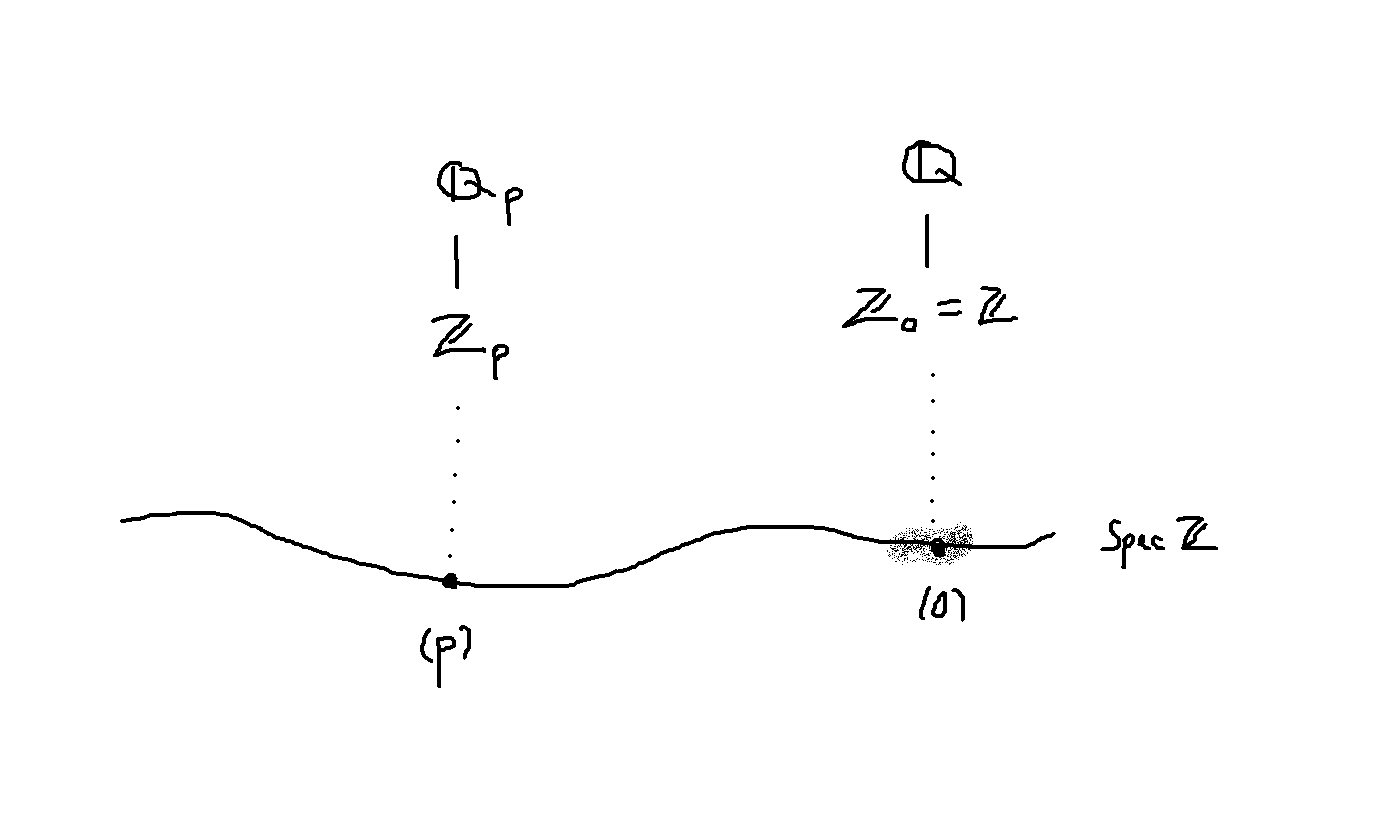
\includegraphics[width=\linewidth,height=\textheight,keepaspectratio]{Figures/places of Spec Z.png}
                                \caption{Local and global points of $\Spec \Z$}
                                \label{fig: local_and_global_points_of_Spec_Z}
                            \end{figure}
                    \end{remark}
                    \begin{definition}[Global models] \label{def: global_models}
                        We want our parametrising scheme, like $\Spec \Z$, to be one where the infinitestimal neighbourhoods (i.e. formal completions) around correspond to spectra of complete discrete valuation rings (for instance, the infinitestimal neighbourhoods $\Spf \Z_p$ around the points $(p) \in |\Spec \Z|$ correspond uniquely to the affine schemes $\Spec \Z_p$), which essentially means we want . We also want $S$ to be connected so that any residue field at a generic point would automatically be the function field of $S$.
                        
                        Let $S$ be base scheme satisfying the above conditions and let $K_0$ be its function field. Then, a \textbf{global model} for an algebraic scheme $X_0$ over $K_0$ shall be a flat and of finite type $S$-scheme $\bbX_0 \to S$. 
                    \end{definition}
                    \begin{remark}[Local-global compatibility] \label{remark: global_to_local_for_models}
                        
                    \end{remark}
                    
                    \begin{definition}[Pointed curves] \label{def: pointed_curves}
                        A \textbf{pointed elliptic curve} is a \textit{finitely presented} and \textit{proper} global model:
                            $$\bbE_0 \to S$$
                        with a distinguised so-called unit section $o_{\bbE_0}: S \to \bbE_0$ of one of the following:
                            \begin{itemize}
                                \item an elliptic curve over a place of $S$,
                                \item a projective nodal cubic curve over a place of $S$ (cf. \cite[\href{https://stacks.math.columbia.edu/tag/0C46}{Tag 0C46}]{stacks}), or
                                \item a projective cuspidal cubic curve over a place of $S$ (a point is a cusp if it corresponds to a non-splitting prime with inertial degree $2$; cf. definition \ref{def: ramification_indices}). 
                            \end{itemize}
                        A fibre of the first kind is said to be over a place of \textbf{good reduction}, whereas fibres over places of the second and third kind are said to be of \textbf{bad reduction}, as one ends up with singularities at those places.
                    \end{definition}
        
        \subsection{Moduli spaces of higher-dimensional abelian varieties; Shimura varieties}
            In a toungue-in-cheek manner, one might say that elliptic curves are nothing but abelian varieties of dimension $1$. One would not be in saying so, but in describing elliptic curves that way, one masks too many important aspects of these objects. This point of view is not entirely myopic and overly simplistic, however, since it does lead to a very fundamental question: do moduli spaces of higher-dimensional abelian varieties admit reasonable descriptions ? To answer this, let us note beforehand that elliptic curves are more than just $1$-dimensional abelian varieties: they admit \textbf{P}olarisations, \say{interesting} \textbf{E}ndomorphism rings, and \textbf{L}evel structures. As moduli stacks of elliptic curves with these extra structures taken into consideration behave quite well, geometrically, speaking, it thus makes sense to consider moduli spaces of abelian varieties that admitting these structures, so-called \textbf{\textit{PEL}-type abelian varieties} (note that elliptic curves admit polarisations trivially, as their automorphism groups - assuming the base field is of characteristic $p \not = 2, 3$ - are isomorphic to $\Z/n\Z$ for $n \in \{2, 4, 6\}$, i.e. finite). 
            
            \subsubsection{The geometry of abelian varieties}
                \begin{definition}[Abelian varieties] \label{def: abelian_varieties}
                    Fix a base scheme $S$. An \textbf{abelian $S$-scheme} is a group $S$-scheme that is smooth, proper, and geometrically connected. An abelian scheme over a field is \textit{a priori} an algebraic variety (in the sense of definition \ref{def: varieties}), so we shall refer to it as an \textbf{abelian variety}.
                \end{definition}
                This might seem like a rather stupid definition: abelian schemes sound like they should be abelian groups in the category of schemes, so why have we not just declared that every abelian group internal to $\Sch_{/S}$ is an abelian scheme ? The reason is two-fold:
                    \begin{enumerate}
                        \item By requiring that our abelian varieties are smooth and proper, we ensure that the machineries of \'etale cohomology are applicable.
                        \item Abelian group objects in $\Sch_{/S}$ can be geometrically very pathological. For instance, the group scheme associating to any commutative $\F_p$-algebra $R$ (for some prime $p$) its group of $n^{th}$ roots of unity is certainly commutative ($\mu_n(R)$, after all, is necessarily a subgroup of $\Z/n\Z$), which is represented by the affine scheme $\Spec \F_p[\zeta]/(\zeta^n - 1)$, is not even smooth in general, as the associated Jacobian vanishses everywhere (cf. definition \ref{def: standard_smoothness}).
                    \end{enumerate}
                As for why we have required abelian schemes to be geometrically connected group schemes in addition to being smooth and proper, this is because we want to make sure that elliptic curves are special cases of abelian schemes (in fact, elliptic curves are precisely abelian schemes of dimension $1$). Additionally, we will see how the connectedness assumption will help us prove that abelian schemes are indeed commutative group schemes.
                
                \begin{remark}[Basic geometric facts about abelian varieties] \label{remark: geometry_of_abelian_varieties}
                    \noindent
                    \begin{itemize}
                        \item \textbf{(Stability under base change):} If $A \to S$ is any ablian scheme and $S' \to S$ is an arbitrary morphism then $A' \cong S' \x_S A$ will also be an abelian scheme, albeit over $S'$ instead of $S$ this time. The proof of this assertion is identical to the argument presented in \ref{remark: moduli_of_elliptic_curves_disambiguations}.
                        \item \textbf{(Moduli stacks of abelian schemes):} For every fixed base scheme $S$, there exists a natural category of abelian $S$-schemes, wherein:
                            \begin{itemize}
                                \item the objects are abelian $S$-schemes, and
                                \item the morphisms are group scheme homomorphisms over $S$.
                            \end{itemize}
                        We will denote it by $(\calM_{n \geq 1})_{/S}$ (where the \say{$n \geq 1$} suggests that abelian of dimensions possibly higher than $1$ are also included); we choose this notation instead of $\Ab(S)$ to avoid confusing abelian schemes with abelian groups internal to schemes. Interestingly, not only is this a full subcategory of the category spanned by (smooth, proper, and geometrically connected) group schemes over $S$, but it is also fibred (in groupoids) over $\Sch_{/S}$ via the evident forgetful functor: the pullback functors between the fibres are simply given by fibred products. Furthermore, the aforementioned fibration:
                            $$(\calM_{n \geq 1})_{/S} \to \Sch_{/S}$$
                        satisfies Zariski, \'etale, fppf, and fpqc descent. 
                        
                        Now, for reasons similar to those discussed in remark \ref{remark: categories_of_elliptic_curves}, we will actually be more interested in the core of the category of abelian $S$-schemes, which we shall denote by $(\calM_{n \geq 1})_{/S}^{\circ}$. This category is (tautologically) fibred in groupoids over $\Sch_{/S}$, and later on, we shall show that certain subcategories of it admits meaningful geometric interpretations.
                        \item \textbf{(Integrality):}
                    \end{itemize}
                \end{remark}
                
                \begin{theorem}[Rigidity of proper flat families] \label{theorem: rigidity_theorem_1}
                    Let $\pi: X \to S$ be a flat and proper morphism of schemes whose local $0^{th}$ cohomologies are all isomorphic to the corresponding residue fields, i.e.:
                        $$\forall s \in |S|: H^0(X_s, \calO_{X_s}) \cong \kappa_s$$
                    Then:
                        \begin{enumerate}
                            \item the canonical map $\pi^{\sharp}: \calO_S \to \pi_*\calO_X$ will be an isomorphism, and
                            \item if $f: S' \to S$ is an affine-schematic morphism and if $\pi': X' \to S'$ is any morphism making the following diagram commutative:
                                $$
                                    \begin{tikzcd}
                                    	{X'} & X \\
                                    	{S'} & S
                                    	\arrow["f", from=2-1, to=2-2]
                                    	\arrow["\pi", from=1-2, to=2-2]
                                    	\arrow["{\pi'}"', from=1-1, to=2-1]
                                    	\arrow[from=1-1, to=1-2]
                                    \end{tikzcd}
                                $$
                            then $\pi': X' \to S'$ shall be constant.
                        \end{enumerate}
                \end{theorem}
                    \begin{proof}
                        \noindent
                        \begin{enumerate}
                            \item 
                            \item 
                        \end{enumerate}             
                    \end{proof}
                \begin{corollary} \label{coro: rigidity_theorem_2}
                    Let $\pi_1: X \to S$ be a flat and proper morphism of schemes whose local $0^{th}$ cohomologies are all isomorphic to the corresponding residue fields, i.e.:
                        $$\forall s \in |S|: H^0(X_s, \calO_{X_s}) \cong \kappa_s$$
                    Additionally, let $\pi_2: Y \to S$ be a separated map fitting into the following commutative diagram:
                        $$
                            \begin{tikzcd}
                            	X && Y \\
                            	& S
                            	\arrow["{\pi_1}"', from=1-1, to=2-2]
                            	\arrow["{\pi_2}", from=1-3, to=2-2]
                            	\arrow["f", from=1-1, to=1-3]
                            \end{tikzcd}
                        $$
                    Suppose now that $f: X \to Y$ is such that the fibre $f_s: X_s \to Y_s$ is constant for some fixed $s \in |S|$. Then, the restriction of $f: X \to Y$ to the connected component of the given point $s \in |S|$ will also be constant.
                \end{corollary}
                    \begin{proof}
                        
                    \end{proof}
                \begin{corollary}[Abelian schemes are abelian groups] \label{coro: abelian_schemes_are_abelian_groups}
                    Abelian schemes are abelian group objects in schemes.
                \end{corollary}
                    \begin{proof}
                        
                    \end{proof}
                    
            \subsubsection{The arithmetic of abelian varieties}
                \paragraph{Polarisations}
                    Let us first take a look at the moduli stack of polarised schemes. For that, however, we will need to say what it means for a line bundle on a scheme to be relatively ample beforehand.
                    
                    The following definition is actually not the most general one (cf. \cite[\href{https://stacks.math.columbia.edu/tag/01VG}{Tag 01VG}]{stacks}), but since abelian schemes are proper by definition, and most base schemes in arithmetic geometry are Noetherian anyway (in fact, most of the time one will simply be working over the spectrum of a field or a very topologically \say{nice} ring like $\Z$ or $\Z_p$), this notion of relative ampleness will suffice.
                    \begin{definition}[Relatively ample line bundles] \label{def: relatively_ample_line_bundles}
                        Let $\pi: X \to S$ be a morphism of schemes, and let $\calL$ be an invertible line bundle over $\calO_{X/S}$. This is said to be \textbf{$\pi$-relatively ample} if and only if:
                            \begin{itemize}
                                \item the base scheme $S$ is Noetherian,
                                \item the structural morphism $\pi: X \to S$ is proper, and
                                \item there exists $s \geq 0$ such that for all $\calF \in \Coh(X_{/S})$, all the higher cohomologies of $\calF \tensor_{\calO_{X/S}} \calL^{\tensor r}$ vanish for $r \geq s$, i.e.:
                                    $$\exists s \geq 0: \forall i > 0: \forall r \geq s: H^i(X_{/S}, \calF \tensor \calL^{\tensor r}) \cong 0$$
                            \end{itemize}
                    \end{definition}
                    \begin{remark}[Base-changing ample line bundles] \label{remark: base_changing_ample_line_bundles}
                        Let $S$ be a Noetherian base scheme, let $\pi: X \to S$ be a proper morphism, and let $f: S' \to S$ be a morphism of finite presentation. Next, consider the following pullback square:
                            $$
                                \begin{tikzcd}
                                	{X'} & X \\
                                	{S'} & S
                                	\arrow["g", from=1-1, to=1-2]
                                	\arrow["{\pi'}"', from=1-1, to=2-1]
                                	\arrow["\pi", from=1-2, to=2-2]
                                	\arrow["f", from=2-1, to=2-2]
                                	\arrow["\lrcorner"{anchor=center, pos=0.125}, draw=none, from=1-1, to=2-2]
                                \end{tikzcd}
                            $$
                        Also, suppose that $\calL$ is a $\pi$-relatively ample line bundle on $X/S$. Now, note that because $f: S' \to S$ is of finite presentation, $\calO_{S'}$ has to be coherent as a $\calO_S$-module, and hence $\calO_{X'}$ is coherent over $\calO_X$ as well. This implies, via the ampleness assumption on $\calL$, that for all coherent $\calO_{X'}$-modules $\calF'$, there exists $s \geq 0$ such that:
                            $$\forall i' > 0: \forall r' \geq s': H^i\left(X'_{/S'}, \calF' \tensor_{\calO_{X'}} \left(\calL^{\tensor r'} \tensor_{\calO_X} \calO_{X'}\right)\right) \cong 0$$
                        This tells us that the obvious base change $g^*\calL \cong \calL \tensor_{\calO_X} \calO_{X'}$ is indeed $\pi'$-relatively ample.
                    \end{remark}
                    
                    We can now define polarisations on schemes:
                    \begin{definition}[Polarisations] \label{def: polarisations}
                        Let $S$ be a Noetherian base scheme and consider a pullback square of the following form:
                            $$
                                \begin{tikzcd}
                                	{X'} & X \\
                                	{S'} & S
                                	\arrow["g", from=1-1, to=1-2]
                                	\arrow["{\pi'}"', from=1-1, to=2-1]
                                	\arrow["\pi", from=1-2, to=2-2]
                                	\arrow["f", from=2-1, to=2-2]
                                	\arrow["\lrcorner"{anchor=center, pos=0.125}, draw=none, from=1-1, to=2-2]
                                \end{tikzcd}
                            $$
                        wherein $\pi: X \to S$ and is flat, proper, and of finite presentation (and hence so is $\pi': X' \to S'$). If $\calL$ and $\calL'$ are relatively ample line bundles on $X/S$ and $X'/S'$ respectively, then one says that they define a \textbf{polarisation between $X/S$ and $X'/S'$} if and only if:
                            $$\calL' \cong g^*\calL$$
                    \end{definition}
                    \begin{remark}[Moduli stackss of polarised schemes] \label{remark: moduli_stacks_of_polarisations}
                        There is a natural fppf-stack of polarised flat proper schemes, which is in fact a substack of the relative Picard stack over $S$, which, we recall, classifies line bundles over $S$-schemes. Specifically, this new fppf-stack, which we will denote by $\Sch_{/S}^{\pol}$, is the restriction of the Picard stack down onto the subcategory of $\Sch_{/S, \fppf}^{\petit}$ spanned by schemes which are flat, proper, and of finite presentation over $S$.
                        
                        Actually, because the base change of ample line bundles along arbitrary morphisms of finite presentation remains ample, $\Sch_{/S}^{\pol}$ also satisfies Zariski, \'etale, and fpqc descent.
                    \end{remark}
                    \begin{remark}[Polarised abelian schemes] \label{remark: moduli_stacks_of_polarisations_on_abelian_schemes}
                        Abelian schemes are smooth and proper by definition, so they span a (non-full) subcategory of the category of schemes which are flat, proper, and of finite presentation over a given base scheme $S$. Should $S$ be Noetherian in addition, one can subsequently construct a natural category of polarised abelian schemes over $S$, which is fibred over $\Sch_{/S}^{\petit}$. By taking the core of this category, one then obtains a moduli space:
                            $$(\Alg\Spc_{/S}^{\pol})^{\circ} \to \Sch_{/S}^{\petit}$$
                        of polarised abelian schemes over $S$. Then, by combining remarks \ref{remark: geometry_of_abelian_varieties} and \ref{remark: moduli_stacks_of_polarisations}, one can show that this moduli space satisfies Zariski, \'etale, fppf, and fpqc descent.
                    \end{remark}
                    
                    \begin{proposition}[Some geometric properties of moduli stacks of polarised schemes] \label{prop: geometric_properties_of_moduli_stacks_of_polarised_schemes}
                        Fix a Noetherian base scheme $S$. 
                            \begin{enumerate}
                                \item There exists a natural and obvious extension of the moduli stack:
                                    $$(\Sch_{/S}^{\pol})^{\circ} \to \Sch_{/S, \fppf}$$
                                to a moduli stack:
                                    $$(\Alg\Spc_{/S}^{\pol})^{\circ} \to \Alg\Spc_{/S, \fppf}^{\petit}$$
                                of \textbf{polarised algebraic spaces}, which is fibred in groupoids over the \textit{small} base category spanned by algebraic spaces fppf over $S$.
                                \item The diagonal:
                                    $$\Delta_{(\Alg\Spc_{/S}^{\pol})^{\circ}}: (\Alg\Spc_{/S}^{\pol})^{\circ}\to (\Alg\Spc_{/S}^{\pol})^{\circ} \x_S (\Alg\Spc_{/S}^{\pol})^{\circ}$$
                                is representable (cf. definition \ref{def: affine_schematic}) as a morphism of stacks on $\Alg\Spc_{/S, \fppf}^{\petit}$. Furthermore, it is separated and of finite presentation.
                                \item As a $(2, 1)$-sheaf on $\Alg\Spc_{/S, \fppf}^{\petit}$, $(\Alg\Spc_{/S}^{\pol})^{\circ}$ preserves limits in $\Alg\Spc_{/S, \fppf}^{\petit}$. 
                            \end{enumerate}
                    \end{proposition}
                        \begin{proof}
                            \noindent
                            \begin{enumerate}
                                \item 
                                \item 
                                \item 
                            \end{enumerate}
                        \end{proof}
                
                \paragraph{Endomorphisms}
                
                \paragraph{Level structures}
            
            \subsubsection{PEL-type Shimura varieties}
                As it turns out, the space parametrising these abelian varieties are Shimura varieties, particularly so-called \textbf{PEL-type Shimura varieties}. These geometric objects are horrifyingly complicated to properly describe in details, however, so let us first take a look at an illustrative example. 
            
                Consider the (absolute) moduli space:
                    $$(\calM_{n = g}^{(d, N)})^{\circ} \to \Sch_{/\Spec \Z[1/N]}$$
                fibred over $\Sch_{/\Spec \Z[1/N]}$, whose fibres over objects $S \in \Sch_{/\Spec \Z[1/N]}$ are the cores of the categories of abelian $S$-schemes $A_{/S}$ which:
                    \begin{itemize}
                        \item are of some fixed dimension $n = g \geq 0$,
                        \item admit a level-$N$ structure $\phi_N: (\Z/N\Z)^{\oplus 2g} \cong A_{/S}[N]$,
                        \item have a polarisation of degree $d^2$.
                    \end{itemize}